
\section{Model dan Aplikasi Aliran Jaringan}
\label{sec:network-flow-models}

Model aliran jaringan digunakan untuk mengoptimalkan pergerakan komoditas, sumber daya, atau informasi melalui suatu jaringan dengan tetap memenuhi kendala kapasitas dan permintaan. Model ini memiliki beragam aplikasi di berbagai bidang:

\begin{itemize}
    \item \textbf{Transportasi dan Logistik}: Mengoptimalkan pergerakan barang melalui rantai pasok sekaligus meminimalkan biaya transportasi.
    \item \textbf{Telekomunikasi}: Mengelola arus lalu lintas data dalam jaringan untuk meminimalkan kemacetan dan latensi.
    \item \textbf{Distribusi Air dan Energi}: Menyeimbangkan aliran air dalam sistem perpipaan atau mengoptimalkan distribusi jaringan listrik untuk meminimalkan kehilangan energi.
    \item \textbf{Penjadwalan Proyek}: Mengalokasikan tugas kepada pekerja sekaligus meminimalkan keterlambatan dan biaya.
    \item \textbf{Masalah Penugasan dan Pencocokan}: Menugaskan sumber daya kepada tugas secara optimal, seperti karyawan kepada proyek atau siswa kepada sekolah.
\end{itemize}

Untuk memulai pembahasan tentang aliran jaringan, pertama-tama kita perlu membahas graf.

\subsection{Graf}

\subsubsection{Graf Tak Berarah}
\begin{definition}{}
Sebuah graf (tak berarah) $G = (V,E)$ didefinisikan oleh himpunan simpul $V$ dan himpunan sisi $E$ yang berisi pasangan-pasangan simpul.
\end{definition}

Sebagai contoh, graf $G$ berikut dapat dideskripsikan oleh:
\begin{itemize}
\item himpunan simpul $V = \{1,2,3,4,5,6\}$ dan
\item himpunan sisi $E = \{(4,6),(4,5), (5,1), (1,2), (2,5), (2,3), (3,4)\}$.
\end{itemize}

\begin{center}
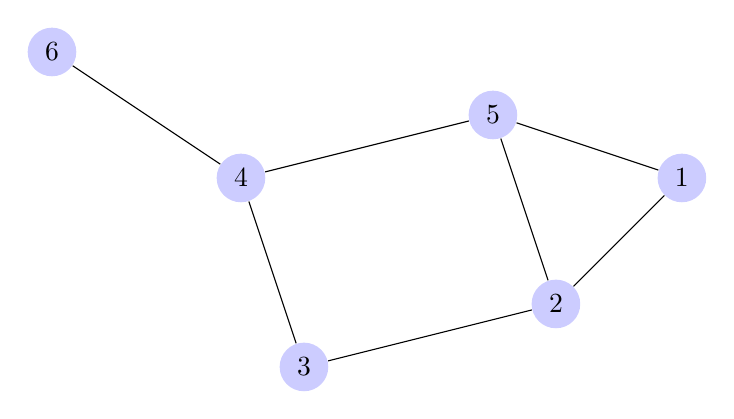
\begin{tikzpicture}
  [scale=.8,auto=left,every node/.style={circle,fill=blue!20}]
  \node (n6) at (1,10) {6};
  \node (n4) at (4,8)  {4};
  \node (n5) at (8,9)  {5};
  \node (n1) at (11,8) {1};
  \node (n2) at (9,6)  {2};
  \node (n3) at (5,5)  {3};

  \foreach \src/\dst in {n6/n4, n4/n5,n5/n1,n1/n2,n2/n5,n2/n3,n3/n4}
    \draw (\src) -- (\dst);

\end{tikzpicture}\par\captionof{figure}{Jaringan tak berarah dengan enam simpul bundar bernomor: sisi-sisinya menghubungkan 6--4, 4--5, 4--3, 5--1, 5--2, 3--2, dan 2--1.}\label{fig:modeling-sums-continued-tikz01}% fig-num-auto

\end{center}

Dalam graf tak berarah, kita tidak membedakan arah sisi. Artinya, untuk dua simpul $i,j \in V$, kita dapat menuliskan $(i,j)$ atau $(j,i)$ secara ekuivalen untuk menyatakan sisi tersebut.

\subsubsection{Graf Berarah}
Sebagai alternatif, kita juga perlu meninjau graf berarah.
\begin{definition}{}{}
Sebuah \emph{graf berarah} (atau digraf) dinotasikan sebagai $G = (V, A)$, dengan $V$ sebagai himpunan simpul dan $A$ sebagai himpunan pasangan simpul terurut yang disebut busur. Jadi, busur menyerupai sisi, tetapi arahnya berpengaruh.
\end{definition}
Sebagai contoh, graf berarah $G$ berikut dapat dideskripsikan oleh
\begin{itemize}
\item himpunan simpul $V = \{1,2,3,4,5,6\}$ dan
\item himpunan busur $ A= \{(4,6),(6,4), (4,5), (5,1), (1,2), (2,5), (2,3), (3,4)\}$.
\end{itemize}
\begin{center}
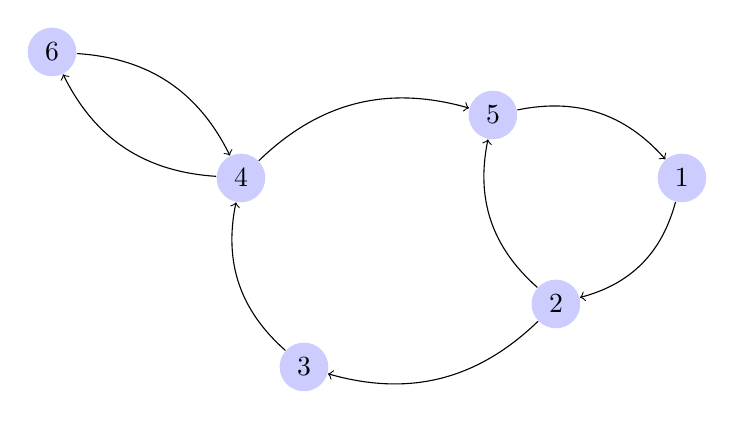
\begin{tikzpicture}
  [scale=.8,auto=left,every node/.style={circle,fill=blue!20}]
  \node (n6) at (1,10) {6};
  \node (n4) at (4,8)  {4};
  \node (n5) at (8,9)  {5};
  \node (n1) at (11,8) {1};
  \node (n2) at (9,6)  {2};
  \node (n3) at (5,5)  {3};

  \foreach \src/\dst in {n6/n4,n4/n6,n4/n5,n5/n1,n1/n2,n2/n5,n2/n3,n3/n4}
	\path[every node/.style={font=\sffamily\small}]
    	(\src) edge[->, bend left] node [left] {} (\dst);

\end{tikzpicture}\par\captionof{figure}{Versi berarah dari jaringan enam simpul yang sama: panah melengkung menunjukkan arah setiap busur, termasuk dua busur berlawanan arah antara simpul 4 dan 6.}\label{fig:modeling-sums-continued-tikz02}% fig-num-auto

\end{center}

\subsection{Contoh: Aliran Berbiaya Minimum dalam Jaringan Transportasi}

\begin{examplewithallcode}{Aliran Jaringan Berbiaya Minimum}
{https://github.com/open-optimization/open-optimization-or-book/blob/master/Intro-Math-Programming/baseText/optimization/optimization-examples/network-flow-excel.xlsx}
{https://github.com/open-optimization/open-optimization-or-book/tree/master/Intro-Math-Programming/baseText/optimization/optimization-examples/network_flow_pulp.ipynb}
{https://github.com/open-optimization/open-optimization-or-book/tree/master/Intro-Math-Programming/baseText/optimization/optimization-examples/network_flow_gurobi.ipynb}
\label{ex:min-cost-flow-warehouses}

Untuk mengilustrasikan masalah aliran jaringan berbiaya minimum, bayangkan sebuah perusahaan yang ingin mengangkut barang dari dua gudang ke dua toko ritel dengan biaya serendah mungkin. Perusahaan dapat mengirimkan barang melalui jaringan rute transportasi; setiap rute memiliki kapasitas dan biaya transportasi per unit tertentu.

Jaringan transportasi tersebut terdiri atas:
\begin{itemize}
    \item \textbf{Dua gudang} (simpul pasokan) yang menyimpan barang:
          \begin{itemize}
              \item \textbf{Gudang 1} dapat memasok paling banyak 20 unit.
              \item \textbf{Gudang 2} dapat memasok paling banyak 30 unit.
          \end{itemize}
    \item \textbf{Dua toko ritel} (simpul permintaan) yang membutuhkan barang:
          \begin{itemize}
              \item \textbf{Toko 1} membutuhkan 25 unit.
              \item \textbf{Toko 2} membutuhkan 25 unit.
          \end{itemize}
    \item Rute transportasi (\textbf{busur}) yang menghubungkan gudang dengan toko; setiap rute memiliki biaya transportasi per unit dan batas kapasitas.
\end{itemize}

\textbf{Representasi Graf}

Jaringan transportasi dapat direpresentasikan sebagai graf berarah \( G = (V, A) \), dengan:

\begin{itemize}
    \item \( V = \{ W_1, W_2, S_1, S_2 \} \) (dua gudang dan dua toko).
    \item \( A = \{(W_1, S_1), (W_1, S_2), (W_2, S_1), (W_2, S_2)\} \) (rute transportasi berarah).
    \item Setiap busur \( (i,j) \) memiliki biaya transportasi \( c_{ij} \) dan kapasitas \( u_{ij} \) tertentu.
\end{itemize}

Data jaringan dirangkum dalam tabel berikut:

    \begin{tabular}{|c|c|c|}
        \hline
        Rute & Biaya per unit ($c_{ij}$) & Kapasitas ($u_{ij}$) \\
        \hline
        Gudang 1 ke Toko 1 & 4 & 15 \\
        Gudang 1 ke Toko 2 & 6 & 10 \\
        Gudang 2 ke Toko 1 & 5 & 20 \\
        Gudang 2 ke Toko 2 & 2 & 20 \\
        \hline
    \end{tabular}
\par\captionof{table}{Biaya dan kapasitas transportasi untuk setiap rute.}\label{tab:modeling-sums-continued-tab01}% tab-num-auto


\modelhead{Model}

Misalkan \( x_{ij} \) menyatakan jumlah barang yang diangkut dari gudang \( i \) ke toko \( j \). Masalah tersebut dirumuskan sebagai:

\begin{align}
\min \quad & 4x_{W_1,S_1} + 6x_{W_1,S_2} + 5x_{W_2,S_1} + 2x_{W_2,S_2}\label{eq:example_objective} \\
    \st \quad
    & x_{W_1,S_1} + x_{W_1,S_2} \leq 20   \tag{Kendala pasokan untuk Gudang 1}\label{eq:supply1} \\
    & x_{W_2,S_1} + x_{W_2,S_2} \leq 30   \tag{Kendala pasokan untuk Gudang 2}\label{eq:supply2} \\
    & x_{W_1,S_1} + x_{W_2,S_1} = 25   \tag{Kendala permintaan untuk Toko 1}\label{eq:demand1} \\
    & x_{W_1,S_2} + x_{W_2,S_2} = 25   \tag{Kendala permintaan untuk Toko 2}\label{eq:demand2} \\
    & 0 \leq x_{ij} \leq u_{ij} &&\quad \text{untuk semua } (i,j) \in A.\label{eq:capacity_constraint_example}
\end{align}

\textbf{Solusi}

Dengan menyelesaikan program linear tersebut, kita memperoleh nilai aliran optimal berikut:

    \begin{tabular}{|c|c|}
        \hline
        Rute & Aliran Optimal ($x_{ij}$) \\
        \hline
        Gudang 1 ke Toko 1 & 15 \\
        Gudang 1 ke Toko 2 & 5 \\
        Gudang 2 ke Toko 1 & 10 \\
        Gudang 2 ke Toko 2 & 20 \\
        \hline
    \end{tabular}
\par\captionof{table}{Aliran optimal pada setiap rute.}\label{tab:modeling-sums-continued-tab02}% tab-num-auto


Biaya minimum total diberikan oleh:
\[
(4 \times 15) + (6 \times 5) + (5 \times 10) + (2 \times 20) = 60 + 30 + 50 + 40 = 180.
\]

\textbf{Interpretasi Solusi}

\begin{itemize}
    \item \textbf{Gudang 1} mengirimkan \textbf{15 unit} ke Toko 1 dan \textbf{5 unit} ke Toko 2.
    \item \textbf{Gudang 2} mengirimkan \textbf{10 unit} ke Toko 1 dan \textbf{20 unit} ke Toko 2.
    \item \textbf{Biaya transportasi total diminimalkan menjadi 180}.
\end{itemize}

Solusi ini memenuhi semua kendala dan memastikan barang diangkut dengan biaya serendah mungkin.

\end{examplewithallcode}
\newpage

\subsection{Masalah Aliran Jaringan Berbiaya Minimum}
\label{sec:min-cost-network-flow}

\emph{Masalah aliran jaringan berbiaya minimum} memperumum model aliran dasar dengan menyertakan kapasitas busur, biaya busur, serta pasokan/permintaan pada simpul. Tujuannya adalah menentukan cara merutekan aliran melalui jaringan dengan biaya serendah mungkin, sekaligus memenuhi permintaan dan menaati semua kendala.

\vspace{0.5em}
\begin{example}{Jaringan Distribusi Amazonian}{}
Amazonian harus mengirimkan barang dari gudang regional besar ke toko ritel lokal melalui pusat distribusi perantara. Setiap gudang memiliki kapasitas pasokan tertentu, setiap toko memiliki permintaan, dan setiap rute menimbulkan biaya transportasi (bahan bakar, waktu, dan tenaga kerja). Amazonian ingin menentukan cara merutekan produk untuk meminimalkan biaya, sambil memastikan permintaan terpenuhi dan tidak ada jalur transportasi yang melampaui kapasitasnya.

\vspace{0.5em}
Gambar di bawah menunjukkan contoh kecil. Terdapat:
\begin{itemize}
\item Dua gudang (W1, W2) dengan pasokan total 50 unit,
\item Dua pusat distribusi (D1, D2),
\item Tiga toko (S1, S2, S3) yang masing-masing membutuhkan 20, 15, dan 15 unit,
\item Biaya busur yang dicantumkan dalam warna hitam,
\item Permintaan/pasokan simpul yang ditampilkan dalam warna biru di samping setiap simpul.
\end{itemize}

\vspace{-1em}
\begin{center}
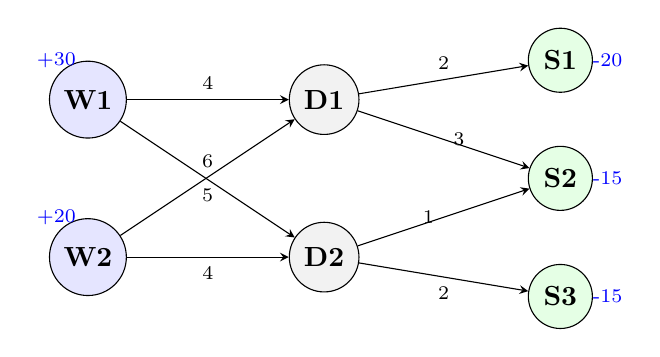
\begin{tikzpicture}[>=stealth, node distance=2cm]

% Gudang
\node[draw, circle, fill=blue!10] (W1) at (0,2) {\textbf{W1}};
\node[draw, circle, fill=blue!10] (W2) at (0,0) {\textbf{W2}};

% Pusat Distribusi
\node[draw, circle, fill=gray!10] (D1) at (3,2) {\textbf{D1}};
\node[draw, circle, fill=gray!10] (D2) at (3,0) {\textbf{D2}};

% Toko
\node[draw, circle, fill=green!10] (S1) at (6,2.5) {\textbf{S1}};
\node[draw, circle, fill=green!10] (S2) at (6,1) {\textbf{S2}};
\node[draw, circle, fill=green!10] (S3) at (6,-0.5) {\textbf{S3}};

% Busur beserta biaya
\draw[->] (W1) -- (D1) node[midway, above] {\scriptsize 4};
\draw[->] (W1) -- (D2) node[midway, below] {\scriptsize 5};
\draw[->] (W2) -- (D1) node[midway, above] {\scriptsize 6};
\draw[->] (W2) -- (D2) node[midway, below] {\scriptsize 4};
\draw[->] (D1) -- (S1) node[midway, above] {\scriptsize 2};
\draw[->] (D1) -- (S2) node[midway, right] {\scriptsize 3};
\draw[->] (D2) -- (S2) node[midway, left] {\scriptsize 1};
\draw[->] (D2) -- (S3) node[midway, below] {\scriptsize 2};

% Pasokan/permintaan
\node[blue] at (-0.4,2.5) {\scriptsize +30};
\node[blue] at (-0.4,0.5) {\scriptsize +20};
\node[blue] at (6.6,2.5) {\scriptsize -20};
\node[blue] at (6.6,1) {\scriptsize -15};
\node[blue] at (6.6,-0.5) {\scriptsize -15};

\end{tikzpicture}\par\captionof{figure}{Jaringan transshipment: simpul pasokan W1 (+30) dan W2 (+20) di sebelah kiri, simpul transshipment D1 dan D2 di tengah, serta simpul permintaan S1 (-20), S2 (-15), dan S3 (-15) di sebelah kanan.}\label{fig:modeling-sums-continued-tikz03}% fig-num-auto

\end{center}

\noindent Masalahnya adalah menentukan jumlah unit yang dikirim melalui setiap rute untuk meminimalkan biaya pengiriman total.

\smallskip \modelhead{Himpunan}
\begin{itemize}
\item \( V \): himpunan simpul dalam jaringan (gudang, pusat distribusi, toko)
\item \( A \): himpunan busur berarah \( (i,j) \) yang merepresentasikan rute pengiriman
\end{itemize}

\smallskip \modelhead{Parameter}
\begin{itemize}
\item \( c_{ij} \): biaya per unit yang dikirim pada busur \( (i, j) \in A \)
\item \( u_{ij} \): kapasitas maksimum busur \( (i, j) \in A \)
\item \( d_i \): pasokan bersih pada simpul \( i \in V \) (positif = pasokan di gudang, negatif = permintaan di toko)
\end{itemize}

\smallskip \modelhead{Variabel} \\
\( x_{ij} \): jumlah aliran yang dikirim melalui busur \( (i, j) \in A \)

\smallskip \modelhead{Model}
\begin{align*}
\min \quad & \sum_{(i,j) \in A} c_{ij} \cdot x_{ij} \\
\st \quad
& \sum_{j : (k,j) \in A} x_{kj} - \sum_{i : (i,k) \in A} x_{ik} = d_k &&\quad \text{untuk semua } k \in V   \tag{keseimbangan aliran} \\
& 0 \leq x_{ij} \leq u_{ij} &&\quad \text{untuk semua } (i,j) \in A   \tag{kendala kapasitas}
\end{align*}

\noindent Masalah ini dapat diselesaikan dengan pemrograman linear, dan tersedia algoritma khusus yang efisien karena strukturnya. Aplikasinya mencakup:
\begin{itemize}
    \item Transportasi barang,
    \item Optimasi rantai pasok,
    \item Penjadwalan dan telekomunikasi.
\end{itemize}
\end{example}

\subsection{Masalah Aliran Jaringan Berbiaya Minimum (Tak Terstruktur)}
Masalah aliran jaringan berbiaya minimum merupakan perluasan masalah aliran jaringan yang tidak hanya mempertimbangkan kapasitas busur, tetapi juga biaya pengiriman aliran melalui busur dan permintaan pada simpul. Tujuannya adalah menemukan aliran berbiaya minimum yang memenuhi permintaan pada simpul dan kendala kapasitas pada busur.

Sebuah jaringan dapat dideskripsikan sebagai graf berarah \( G = (V, A) \), dengan \( V \) sebagai himpunan simpul dan \( A \) sebagai himpunan busur. Setiap busur \( (i, j) \in A \) memiliki kapasitas \( u_{ij} \) dan biaya \( c_{ij} \). Setiap simpul \( i \in V\) memiliki permintaan \( d_i \), yang dapat bernilai positif, negatif, atau nol. Permintaan positif berarti simpul membutuhkan aliran sebanyak nilai tersebut, permintaan negatif berarti simpul memasok aliran sebanyak nilai mutlaknya, dan permintaan nol berarti simpul tidak membutuhkan maupun memasok aliran. Perhatikan bahwa konvensi tanda pada bagian ini berlawanan dengan contoh sebelumnya: di sini nilai positif berarti permintaan dan persamaan keseimbangan menggunakan aliran masuk dikurangi aliran keluar. Kedua konvensi tetap konsisten di dalam modelnya masing-masing.

Sebagai contoh, tinjau:
Himpunan simpul diberikan oleh:
\[
V = \{ a, b, c, d, e, f, g, h \}
\]
Himpunan busur berarah adalah:
\[
A = \{ (b,a), (a,c), (d,b), (b,e), (c,e), (c,f), (h,d), (g,e), (e,h), (g,f) \}
\]
\begin{center}
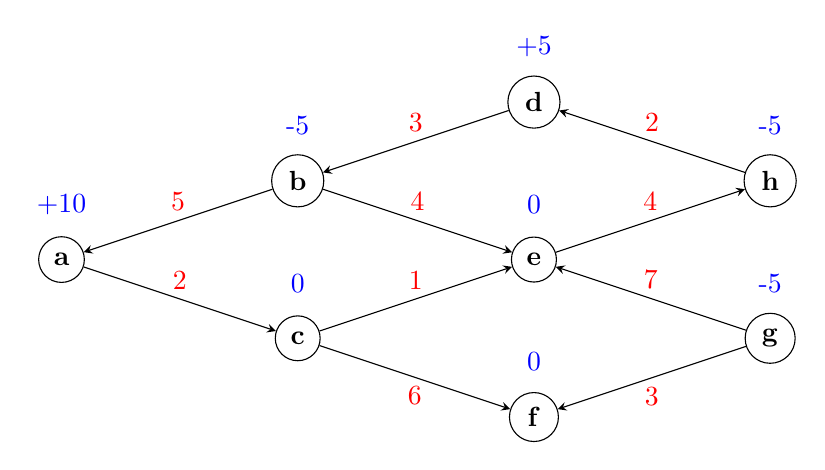
\begin{tikzpicture}[>=stealth, node distance=3cm]

    % Simpul (dilingkari)
    \node[draw, circle] (a) at (0,6) {\textbf{a}};
    \node[draw, circle] (b) at (3,7) {\textbf{b}};
    \node[draw, circle] (c) at (3,5) {\textbf{c}};
    \node[draw, circle] (d) at (6,8) {\textbf{d}};
    \node[draw, circle] (e) at (6,6) {\textbf{e}};
    \node[draw, circle] (f) at (6,4) {\textbf{f}};
    \node[draw, circle] (g) at (9,5) {\textbf{g}};
    \node[draw, circle] (h) at (9,7) {\textbf{h}};

    % Anotasi aliran bersih (di atas simpul, berwarna biru)
    \node[blue] at (0,6.7) {+10};
    \node[blue] at (3,7.7) {-5};
    \node[blue] at (3,5.7) {0};
    \node[blue] at (6,8.7) {+5};
    \node[blue] at (6,6.7) {0};
    \node[blue] at (6,4.7) {0};
    \node[blue] at (9,5.7) {-5};
    \node[blue] at (9,7.7) {-5};

    % Sisi beserta biaya (berwarna merah)
    \draw[->] (b) -- (a) node[midway, above,  red] {5};
    \draw[->] (a) -- (c) node[midway, above,  red] {2};
    \draw[->] (d) -- (b) node[midway, above,  red] {3};
    \draw[->] (b) -- (e) node[midway, above,  red] {4};
    \draw[->] (c) -- (e) node[midway, above,  red] {1};
    \draw[->] (c) -- (f) node[midway, below,  red] {6};
    \draw[->] (h) -- (d) node[midway, above,  red] {2};
    \draw[->] (g) -- (e) node[midway, above,  red] {7};
    \draw[->] (e) -- (h) node[midway, above,  red] {4};
    \draw[->] (g) -- (f) node[midway, below,  red] {3};
    
\end{tikzpicture}\par\captionof{figure}{Jaringan berarah dengan delapan simpul berlabel a sampai h yang tersusun dari kiri ke kanan.}\label{fig:modeling-sums-continued-tikz04}% fig-num-auto

\end{center}
\begin{table}[h]
    \centering
    \begin{minipage}{0.45\textwidth}
        \centering
        \begin{tabular}{|c|c|c|}
            \hline
            \textbf{Dari} & \textbf{Ke} & \textbf{Biaya} \\
            \hline
            b & a & {\color{red} 5 }\\
            a & c & {\color{red}2} \\
            d & b & {\color{red}3 }\\
            b & e & {\color{red}4 }\\
            c & e & {\color{red}1 }\\
            c & f & {\color{red}6 }\\
            h & d & {\color{red}2 }\\
            g & e & {\color{red}7 }\\
            e & h & {\color{red}4 }\\
            g & f & {\color{red}3} \\
            \hline
        \end{tabular}
        \caption{Biaya Busur dalam Masalah Aliran Jaringan}
        \label{tab:arc_costs}
    \end{minipage}
    \hfill
    \begin{minipage}{0.45\textwidth}
        \centering
        \begin{tabular}{|c|c|}
            \hline
            \textbf{Simpul} & \textbf{Aliran Bersih} \\
            \hline
            a & {\color{blue}+10} \\
            b & {\color{blue}-5} \\
            c & {\color{blue}0} \\
            d & {\color{blue}+5 }\\
            e & {\color{blue}0} \\
            f & {\color{blue}0} \\
            g & {\color{blue}-5} \\
            h & {\color{blue}-5} \\
            \hline
        \end{tabular}
        \caption{Aliran Bersih pada Setiap Simpul}
        \label{tab:net_flow}
    \end{minipage}
\end{table}
Masalah aliran jaringan berbiaya minimum dapat didefinisikan sebagai berikut: diberikan jaringan \( G = (V, A) \), kapasitas \( u_{ij} \) dan biaya \( c_{ij} \) pada busur, serta permintaan \( d_i \) pada simpul, tentukan aliran \( x_{ij} \) pada busur yang meminimalkan biaya total aliran sambil memenuhi permintaan pada simpul dan kendala kapasitas pada busur.

\modelhead{Himpunan}
\begin{itemize}
\item \( V \): Himpunan simpul dalam jaringan.
\item \( A \): Himpunan busur dalam jaringan.
\end{itemize}

\modelhead{Parameter}
\begin{itemize}
\item \( u_{ij} \): Kapasitas busur \( (i, j) \in A \).
\item \( c_{ij} \): Biaya per unit aliran pada busur \( (i, j) \in A \).
\item \( d_i \): Permintaan bersih pada simpul \( i \in V \) (positif = permintaan, negatif = pasokan).
\end{itemize}

\modelhead{Variabel}
\begin{itemize}
\item \( x_{ij} \): Aliran pada busur \( (i, j) \in A \).
\end{itemize}

\modelhead{Model}
Masalah aliran jaringan berbiaya minimum dapat dirumuskan sebagai masalah pemrograman linear berikut:

\begin{align*}
\min \quad & \sum_{(i, j) \in A} c_{ij} x_{ij} \\
\st        & \sum_{i:(i, k) \in A} x_{ik} - \sum_{j:(k, j) \in A} x_{kj} = d_k &&\quad \text{untuk semua } k \in V \\
& 0 \leq x_{ij} \leq u_{ij} &&\quad \text{untuk semua } (i, j) \in A
\end{align*}

\modelhead{Fungsi Tujuan}
- Fungsi tujuan meminimalkan biaya total aliran.

\modelhead{Kendala}
- Konservasi Aliran: Kelompok kendala pertama memastikan bahwa aliran yang masuk ke setiap simpul dikurangi aliran yang keluar dari simpul tersebut sama dengan permintaan pada simpul itu.

- Kendala Kapasitas: Kelompok kendala kedua memastikan bahwa aliran pada setiap busur tidak melampaui kapasitasnya.

Masalah aliran jaringan berbiaya minimum banyak digunakan dalam perencanaan transportasi, logistik rantai pasok, dan penjadwalan produksi, dengan tujuan mengalokasikan sumber daya secara efisien dengan biaya serendah mungkin.

\subsection{Aliran Maksimum}
\label{sec:max-flow}

Masalah aliran maksimum merupakan masalah mendasar dalam riset operasi dan ilmu komputer, dengan aplikasi di berbagai bidang. Masalah ini mencari jumlah aliran maksimum yang dapat dikirimkan dari sebuah simpul sumber ke sebuah simpul tujuan dalam suatu jaringan, tanpa melampaui kapasitas masing-masing busur dan dengan memastikan bahwa aliran pada setiap busur tidak negatif. Masalah ini muncul dalam banyak situasi nyata. Dalam transportasi, misalnya, masalah ini dapat digunakan untuk menemukan jumlah maksimum barang yang dapat diangkut dari pabrik ke gudang; dalam telekomunikasi, masalah ini dapat digunakan untuk menemukan jumlah maksimum data yang dapat dikirim dari satu server ke server lain. Aplikasi lainnya mencakup optimasi rantai pasok, distribusi air, dan optimasi jaringan tenaga listrik. Pada bagian ini, kita akan mendeskripsikan rumusan pemrograman linear untuk masalah aliran jaringan.

Sebuah jaringan dapat dideskripsikan sebagai graf berarah \( G = (V, A) \), dengan \( V \) sebagai himpunan simpul dan \( A \) sebagai himpunan busur. Setiap busur \( (i, j) \in A \) memiliki kapasitas \( u_{ij} \), yaitu jumlah maksimum aliran yang dapat melewati busur dari simpul \( i \) ke simpul \( j \).

Masalah aliran jaringan dapat didefinisikan sebagai berikut: diberikan sebuah jaringan \( G = (V, A) \), simpul sumber \( s \), simpul tujuan \( t \), dan kapasitas \( u_{ij} \) pada setiap busur, temukan aliran maksimum dari \( s \) ke \( t \) yang memenuhi kendala kapasitas.

Sebagai contoh, tinjau graf berarah berikut dengan kapasitas pada busurnya.
\begin{center}
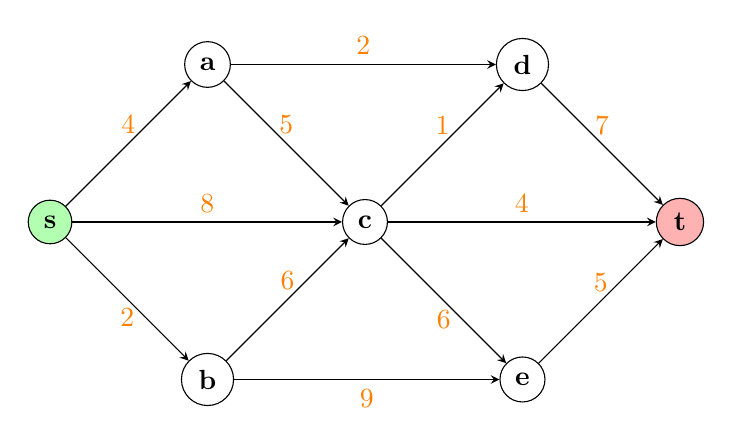
\begin{tikzpicture}[>=stealth, node distance=2cm]

    % Simpul dengan gaya tertentu
    \node[fill=green,
         fill opacity = 0.3, draw, circle,  text opacity=1] (s) at (0,2) {\textbf{s}};
    \node[draw, circle] (a) at (2,4) {\textbf{a}};
    \node[draw, circle] (b) at (2,0) {\textbf{b}};
    \node[draw, circle] (c) at (4,2) {\textbf{c}};
    \node[draw, circle] (d) at (6,4) {\textbf{d}};
    \node[draw, circle] (e) at (6,0) {\textbf{e}};
    \node[fill=red,
         fill opacity = 0.3, draw, circle,  text opacity=1] (t) at (8,2) {\textbf{t}};

    % Sisi beserta kapasitas (jingga, tegak)
    \draw[->] (s) -- (a) node[midway, above, text=orange] {4};
    \draw[->] (s) -- (c) node[midway, above, text=orange] {8};
    \draw[->] (s) -- (b) node[midway, below, text=orange] {2};
    \draw[->] (a) -- (c) node[midway, above, text=orange] {5};
    \draw[->] (a) -- (d) node[midway, above, text=orange] {2};
    \draw[->] (c) -- (d) node[midway, above, text=orange] {1};
    \draw[->] (c) -- (t) node[midway, above, text=orange] {4};
    \draw[->] (c) -- (e) node[midway, below, text=orange] {6};
    \draw[->] (b) -- (c) node[midway, above, text=orange] {6};
    \draw[->] (b) -- (e) node[midway, below, text=orange] {9};
    \draw[->] (d) -- (t) node[midway, above, text=orange] {7};
    \draw[->] (e) -- (t) node[midway, above, text=orange] {5};

\end{tikzpicture}
\end{center}

\begin{examplewithallcode}{Jaringan Transit Maskapai: Memaksimalkan Jumlah Penumpang}
{https://github.com/open-optimization/open-optimization-or-book/blob/master/Intro-Math-Programming/baseText/optimization/optimization-examples/airline-maxflow-excel.xlsx}
{https://github.com/open-optimization/open-optimization-or-book/tree/master/Intro-Math-Programming/baseText/optimization/optimization-examples/airline_maxflow_pulp.ipynb}
{https://github.com/open-optimization/open-optimization-or-book/tree/master/Intro-Math-Programming/baseText/optimization/optimization-examples/airline_maxflow_gurobi.ipynb}
Sebuah maskapai berusaha merutekan ulang sebanyak mungkin penumpang yang terlantar dari kota asal (\(s\)) ke kota tujuan (\(t\)) dengan menggunakan jaringan penerbangan penghubung. Setiap penerbangan memiliki jumlah kursi tersedia yang diketahui, dan penumpang dapat berpindah pesawat di bandara perantara. Tujuannya adalah menentukan jumlah maksimum penumpang yang dapat dirutekan dari asal ke tujuan dengan memanfaatkan kapasitas kursi yang tersedia dan menaati rute penerbangan.

\vspace{0.5em}
Jaringan tersebut mencakup:
\begin{itemize}
    \item Bandara asal \(s\),
    \item Hub perantara: \(a, b, c\),
    \item Bandara transit regional: \(d, e\),
    \item Bandara tujuan akhir \(t\),
    \item Segmen penerbangan berarah (busur) dengan ketersediaan kursi yang diketahui.
\end{itemize}

\smallskip \modelhead{Himpunan dan Parameter}
\begin{itemize}
    \item \( V = \{s, a, b, c, d, e, t\} \): himpunan bandara.
    \item \( A = \{(s,a), (s,b), (s,c), (a,c), (a,d), (b,c), (b,e), (c,d), (c,e), (c,t), (d,t), (e,t)\} \): himpunan segmen penerbangan.
    \item \( u_{ij} \): jumlah kursi yang tersedia pada penerbangan dari bandara \( i \) ke \( j \), untuk semua $(i,j) \in A$.
\end{itemize}

\smallskip \modelhead{Variabel} \\
\( x_{ij} \): jumlah penumpang yang ditugaskan terbang dari bandara \( i \) ke \( j \), untuk semua $(i,j) \in A$

\smallskip \modelhead{Model}
\begin{align*}
\max \quad & x_{sa} + x_{sb} + x_{sc} \\
\st \quad
& x_{ac} + x_{ad} - x_{sa} = 0 \\
& x_{bc} + x_{be} - x_{sb} = 0 \\
& x_{cd} + x_{ce} + x_{ct} - x_{ac} - x_{bc} - x_{sc} = 0 \\
& x_{dt} - x_{ad} - x_{cd} = 0 \\
& x_{et} - x_{be} - x_{ce} = 0 \\
& 0 \leq x_{sa} \leq 4,\quad 0 \leq x_{sb} \leq 2,\quad 0 \leq x_{sc} \leq 8 \\
& 0 \leq x_{ac} \leq 5,\quad 0 \leq x_{ad} \leq 2 \\
& 0 \leq x_{bc} \leq 6,\quad 0 \leq x_{be} \leq 9 \\
& 0 \leq x_{cd} \leq 1,\quad 0 \leq x_{ce} \leq 3,\quad 0 \leq x_{ct} \leq 4 \\
& 0 \leq x_{dt} \leq 7,\quad 0 \leq x_{et} \leq 5.
\end{align*}
Lima persamaan pertama menegakkan keseimbangan aliran di bandara
perantara $a,b,c,d,e$; batas-batas berikutnya menyatakan jumlah kursi yang
tersedia pada setiap segmen penerbangan.
\newpage
Dalam bentuk notasi penjumlahan yang ringkas, kita memperoleh

$$
\begin{aligned}
\max \quad & \sum_{j \in V : (s,j) \in A} x_{sj} \\
\st        & \sum_{j \in V : (k,j) \in A} x_{kj} - \sum_{i \in V : (i,k) \in A} x_{ik} = 0 &&\quad \text{untuk semua } k \in V \setminus \{s,t\} \\
           & 0 \leq x_{ij} \leq u_{ij} &&\quad \text{untuk semua } (i,j) \in A
\end{aligned}
$$

\vspace{0.5em}
\noindent Model ini membantu maskapai menentukan penugasan penumpang ke segmen penerbangan sehingga kapasitas jaringan yang tersedia dimanfaatkan semaksimal mungkin. Model ini terutama berguna dalam situasi gangguan seperti:
\begin{itemize}
    \item pembatalan akibat cuaca buruk,
    \item perutean ulang darurat akibat masalah pemeliharaan,
    \item acara dengan permintaan tinggi yang memerlukan perutean tambahan sementara.
\end{itemize}

Kerangka yang sama dapat diperluas untuk mencakup prioritas, jendela waktu, atau biaya pemesanan ulang.
\end{examplewithallcode}

Solusinya ditunjukkan pada graf berikut dengan nilai aliran dicetak tebal. Aliran totalnya adalah 12.
\begin{center}
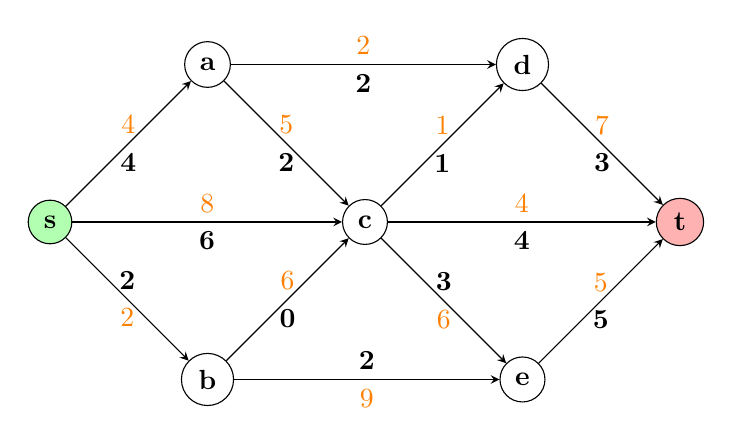
\begin{tikzpicture}[>=stealth, node distance=2cm]

    % Simpul dengan gaya tertentu
    \node[draw, circle, fill=green,
         fill opacity = 0.3,  text opacity=1] (s) at (0,2) {\textbf{s}};
    \node[draw, circle] (a) at (2,4) {\textbf{a}};
    \node[draw, circle] (b) at (2,0) {\textbf{b}};
    \node[draw, circle] (c) at (4,2) {\textbf{c}};
    \node[draw, circle] (d) at (6,4) {\textbf{d}};
    \node[draw, circle] (e) at (6,0) {\textbf{e}};
    \node[ fill=red,
         fill opacity = 0.3, draw, circle,  text opacity=1] (t) at (8,2) {\textbf{t}};

    % Sisi beserta kapasitas (jingga, tegak) dan aliran (hitam tebal, di bawah)
    \draw[->] (s) -- (a) node[midway, above, text=orange] {4}
                         node[midway, below, text=black] {\textbf{4}};
    \draw[->] (s) -- (c) node[midway, above, text=orange] {8}
                         node[midway, below, text=black] {\textbf{6}};
    \draw[->] (s) -- (b) node[midway, below, text=orange] {2}
                         node[midway, above, text=black] {\textbf{2}};
    
    \draw[->] (a) -- (c) node[midway, above, text=orange] {5}
                         node[midway, below, text=black] {\textbf{2}};
    \draw[->] (a) -- (d) node[midway, above, text=orange] {2}
                         node[midway, below, text=black] {\textbf{2}};

    \draw[->] (c) -- (d) node[midway, above, text=orange] {1}
                         node[midway, below, text=black] {\textbf{1}}; % Disesuaikan agar menaati kapasitas
    \draw[->] (c) -- (t) node[midway, above, text=orange] {4}
                         node[midway, below, text=black] {\textbf{4}};
    \draw[->] (c) -- (e) node[midway, below, text=orange] {6}
                         node[midway, above, text=black] {\textbf{3}};

    \draw[->] (b) -- (c) node[midway, above, text=orange] {6}
                         node[midway, below, text=black] {\textbf{0}};
    \draw[->] (b) -- (e) node[midway, below, text=orange] {9}
                         node[midway, above, text=black] {\textbf{2}};

    \draw[->] (d) -- (t) node[midway, above, text=orange] {7}
                         node[midway, below, text=black] {\textbf{3}};
    \draw[->] (e) -- (t) node[midway, above, text=orange] {5}
                         node[midway, below, text=black] {\textbf{5}};

\end{tikzpicture}
\end{center}

Masalah aliran maksimum dapat dituliskan secara matematis sebagai berikut.\\

\modelhead{Himpunan}
\begin{itemize}
\item \( V \): Himpunan simpul dalam jaringan.
\item \( A \): Himpunan busur dalam jaringan.
\end{itemize}

\modelhead{Parameter}
\begin{itemize}
\item \( u_{ij} \): Kapasitas busur \( (i, j) \in A \), yaitu jumlah maksimum aliran yang dapat melewati busur dari simpul \( i \) ke simpul \( j \).
\item \( s \): Simpul sumber.
\item \( t \): Simpul tujuan.
\end{itemize}

\modelhead{Variabel}
\begin{itemize}
\item \( x_{ij} \): Aliran pada busur \( (i, j) \in A \).
\end{itemize}

\Needspace{10\baselineskip}
\modelhead{Model}
Masalah aliran jaringan dapat dirumuskan sebagai masalah pemrograman linear berikut:

\begin{align*}
\max \quad & \sum_{j:(s, j) \in A} x_{sj} \\
\st        & \sum_{i:(i, k) \in A} x_{ik} - \sum_{j:(k, j) \in A} x_{kj} = 0 &&\quad \text{untuk semua } k \in V \setminus \{s, t\} \\
%& \sum_{j:(s, j) \in A} x_{sj} - \sum_{j:(j, s) \in A} x_{js} = \sum_{j:(j, t) \in A} x_{jt} - \sum_{j:(t, j) \in A} x_{tj} \\
& 0 \leq x_{ij} \leq u_{ij} &&\quad \text{untuk semua } (i, j) \in A
\end{align*}

\modelhead{Fungsi Tujuan}
- Fungsi tujuan memaksimalkan aliran total dari simpul sumber \( s \) ke simpul tujuan \( t \).

\modelhead{Kendala}
- Keseimbangan Aliran: Kelompok kendala pertama memastikan bahwa aliran yang masuk ke setiap simpul sama dengan aliran yang keluar, kecuali pada simpul sumber dan simpul tujuan.

- Kendala Kapasitas: Kelompok kendala kedua memastikan bahwa aliran pada setiap busur tidak melampaui kapasitasnya.

Kita akan membahas dualitas nanti. Namun, dualitas merupakan konsep yang membantu membentuk batas untuk suatu masalah.
Untuk masalah khusus ini, kita dapat menganggap dual sebagai suatu \emph{cut} atau pemotongan pada graf---sesuatu yang memisahkan $s$ dari $t$. Sebagai contoh:
\begin{center}
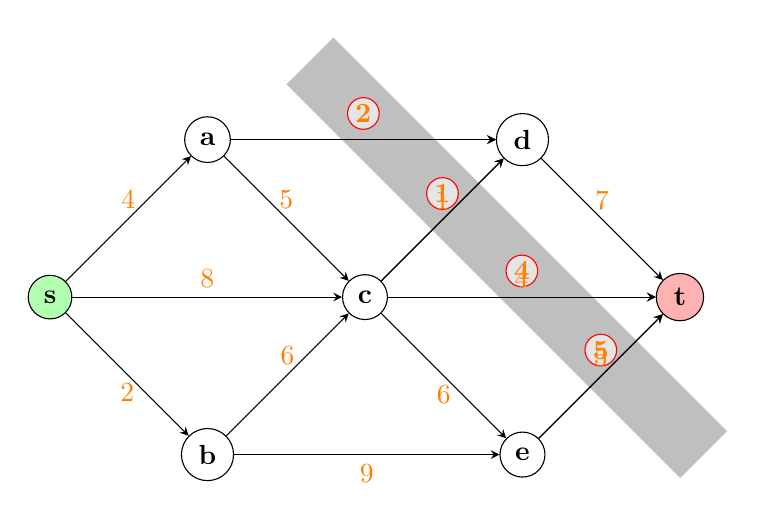
\begin{tikzpicture}[>=stealth, node distance=2cm]

    % Simpul dengan gaya tertentu
    \node[fill=green,
         fill opacity = 0.3, draw, circle,  text opacity=1] (s) at (0,2) {\textbf{s}};
    \node[draw, circle] (a) at (2,4) {\textbf{a}};
    \node[draw, circle] (b) at (2,0) {\textbf{b}};
    \node[draw, circle] (c) at (4,2) {\textbf{c}};
    \node[draw, circle] (d) at (6,4) {\textbf{d}};
    \node[draw, circle] (e) at (6,0) {\textbf{e}};
    \node[fill=red,
         fill opacity = 0.3, draw, circle,  text opacity=1] (t) at (8,2) {\textbf{t}};

\draw[line width=24pt, gray, opacity=0.5] (3.3,5) -- (8.3,0);

    % Sisi beserta kapasitas (jingga, tegak)
    \draw[->] (s) -- (a) node[midway, above, text=orange] {4};
    \draw[->] (s) -- (c) node[midway, above, text=orange] {8};
    \draw[->] (s) -- (b) node[midway, below, text=orange] {2};
    \draw[->] (a) -- (c) node[midway, above, text=orange] {5};
    \draw[->] (a) -- (d) node[ midway, above, text=orange] {2};
\draw[->] (a) -- (d) node[midway, above] {
    \tikz[baseline]{
        \node[draw=red, fill=gray!20, circle, inner sep=1pt, text = orange] {\textbf{2}};
    }
};
\draw[->] (c) -- (d) node[midway, above] {
    \tikz[baseline]{
        \node[draw=red, fill=gray!20, circle, inner sep=1pt, text = orange] {\textbf{1}};
    }
};
\draw[->] (c) -- (t) node[midway, above] {
    \tikz[baseline]{
        \node[draw=red, fill=gray!20, circle, inner sep=1pt, text = orange] {\textbf{4}};
    }
};
\draw[->] (e) -- (t) node[midway, above] {
    \tikz[baseline]{
        \node[draw=red, fill=gray!20, circle, inner sep=1pt, text = orange] {\textbf{5}};
    }
};
    \draw[->] (c) -- (d) node[midway, above, text=orange] {1};
    \draw[->] (c) -- (t) node[midway, above, text=orange] {4};
    \draw[->] (c) -- (e) node[midway, below, text=orange] {6};
    \draw[->] (b) -- (c) node[midway, above, text=orange] {6};
    \draw[->] (b) -- (e) node[midway, below, text=orange] {9};
    \draw[->] (d) -- (t) node[midway, above, text=orange] {7};
    \draw[->] (e) -- (t) node[midway, above, text=orange] {5};

\end{tikzpicture}
\end{center}
Busur-busur yang dipilih membentuk sebuah cut yang memisahkan $s$ dari $t$. Jumlah bobotnya adalah $2 + 1 + 4 + 5 = 12$, sehingga tidak mungkin ada aliran lebih dari 12 unit dari $s$ ke $t$.

Batas ini merupakan salah satu bentuk \emph{dualitas}. Kita akan mempelajari konsep tersebut lebih lanjut pada bab-bab berikutnya. Dualitas ini dirangkum dalam teorema berikut.

\begin{theorem}{}
Besarnya aliran maksimum sama dengan ukuran cut minimum.
\end{theorem}

%
%
\subsection{Aliran Multikomoditas Berbiaya Minimum dengan Kendala Keutuhan}
\label{sec:multicommodity-flow}

Masalah aliran jaringan multikomoditas berbiaya minimum merupakan perumuman masalah aliran jaringan berbiaya minimum yang mempertimbangkan banyak komoditas yang mengalir melalui jaringan. Setiap komoditas memiliki permintaannya sendiri pada setiap simpul dan biayanya sendiri pada setiap busur. Tujuannya adalah menemukan aliran bilangan bulat berbiaya minimum yang memenuhi permintaan semua komoditas pada simpul dan kendala kapasitas pada busur.

Sebuah jaringan dapat dideskripsikan sebagai graf berarah \( G = (N, A) \), dengan \( N \) sebagai himpunan simpul dan \( A \) sebagai himpunan busur. Setiap busur \( (i, j) \in A \) memiliki kapasitas \( u_{ij} \). Setiap komoditas \( k \) memiliki permintaan \( d_{ik} \) pada setiap simpul \( i \in N \) dan biaya \( c_{ijk} \) pada setiap busur \( (i, j) \in A \).

Masalah aliran jaringan multikomoditas berbiaya minimum dapat didefinisikan sebagai berikut: diberikan jaringan \( G = (N, A) \), kapasitas \( u_{ij} \) pada busur, serta permintaan \( d_{ik} \) dan biaya \( c_{ijk} \) untuk setiap komoditas \( k \), tentukan aliran bilangan bulat \( f_{ijk} \) pada busur untuk setiap komoditas \( k \) yang meminimalkan biaya total aliran, sambil memenuhi permintaan semua komoditas pada simpul dan kendala kapasitas pada busur.

\modelhead{Himpunan}
\begin{itemize}
\item \( N \): Himpunan simpul dalam jaringan.
\item \( A \): Himpunan busur dalam jaringan.
\item \( K \): Himpunan komoditas.
\end{itemize}
%
\modelhead{Parameter}
\begin{itemize}
\item \( u_{ij} \): Kapasitas busur \( (i, j) \in A \).
\item \( c_{ijk} \): Biaya per unit aliran komoditas \( k \) pada busur \( (i, j) \in A \).
\item \( d_{ik} \): Permintaan komoditas \( k \) pada simpul \( i \in N \).
\end{itemize}
%
\modelhead{Variabel}
\begin{itemize}
\item \( f_{ijk} \): Aliran komoditas \( k \) pada busur \( (i, j) \in A \).
\end{itemize}
%
\modelhead{Model}
Masalah aliran jaringan multikomoditas berbiaya minimum dapat dirumuskan sebagai masalah pemrograman linear bilangan bulat berikut:

\begin{align*}
\min \quad & \sum_{k \in K} \sum_{(i, j) \in A} c_{ijk} f_{ijk} \\
\st        & \sum_{k \in K} f_{ijk} \leq u_{ij} &&\quad \text{untuk semua } (i, j) \in A \\
& \sum_{j:(j, i) \in A} f_{jik} - \sum_{j:(i, j) \in A} f_{ijk} = d_{ik} &&\quad \text{untuk semua } i \in N, \; \forall k \in K \\
& f_{ijk} \in \mathbb{Z}_{\geq 0} &&\quad \text{untuk semua } (i, j) \in A, \; \forall k \in K
\end{align*}

\modelhead{Fungsi Tujuan}
Fungsi tujuan meminimalkan biaya total aliran, yang dijumlahkan atas semua komoditas dan semua busur.

\modelhead{Kendala}
\begin{itemize}
\item \textbf{Kendala Kapasitas:} Kelompok kendala pertama memastikan bahwa aliran total pada setiap busur (dijumlahkan atas semua komoditas) tidak melampaui kapasitasnya.
\item \textbf{Konservasi Aliran:} Kelompok kendala kedua memastikan bahwa, untuk setiap komoditas, aliran bersih yang masuk ke setiap simpul sama dengan permintaan komoditas tersebut pada simpul itu.
\item \textbf{Kendala Keutuhan:} Kelompok kendala ketiga memastikan bahwa aliran setiap komoditas pada setiap busur berupa bilangan bulat tak negatif.
\end{itemize}


\begin{examplewithallcode}{Aliran jaringan multikomoditas}
{}
{https://github.com/open-optimization/open-optimization-or-book/tree/master/Intro-Math-Programming/baseText/optimization/optimization-examples/multicommodity_flow_pulp.ipynb}
{https://github.com/open-optimization/open-optimization-or-book/tree/master/Intro-Math-Programming/baseText/optimization/optimization-examples/multicommodity_flow_gurobi.ipynb}
\label{ex:multicommodity-network-flow}

Tinjau jaringan kecil dengan 4 simpul dan 4 busur yang mengangkut 2 komoditas. Setiap busur memiliki kapasitas bersama, sedangkan setiap komoditas memiliki biaya per unitnya sendiri pada setiap busur dan pola pasokan/permintaannya sendiri pada setiap simpul (nilai negatif menunjukkan pasokan, sedangkan nilai positif menunjukkan permintaan).
\begin{verbatim}
# Data contoh
nodes = [1, 2, 3, 4]
arcs = [(1, 2), (1, 3), (2, 4), (3, 4)]
commodities = [1, 2]
capacities = {(1, 2): 20, (1, 3): 15, (2, 4): 25, (3, 4): 20}
costs = {(1, 2, 1): 2, (1, 2, 2): 3, (1, 3, 1): 3,
         (1, 3, 2): 2, (2, 4, 1): 1, (2, 4, 2): 2,
         (3, 4, 1): 2, (3, 4, 2): 1}
demands = {(1, 1): -10, (1, 2): -5, (2, 1): 0, (2, 2): 0,
           (3, 1): 0,   (3, 2): 0,  (4, 1): 10, (4, 2): 5}
\end{verbatim}

Dua gambar di bawah menunjukkan jaringan masukan (kiri) dan penugasan aliran optimal (kanan). Setiap busur diberi label aliran komoditas yang dibawanya; kendala kapasitas busur mengharuskan jumlah aliran komoditas tersebut tidak melampaui kapasitas busur.

% --- Rekonstruksi TikZ dari gambar networkx: multi-network-flow-data.png ---
% Tidak mengambang (blok ini berada di dalam kotak examplewithallcode berbingkai,
% yang tidak dapat memuat float figure/table).
\begin{center}
\begin{tikzpicture}[
    every node/.style={circle, draw=black, fill=cyan!40, minimum size=8mm, inner sep=1pt, font=\small},
    every edge/.style={draw, thick},
    >=Stealth,
    node distance=2.5cm and 3cm
  ]
  % Posisi simpul mengikuti tata letak networkx: 1 di tengah atas, 2 di kanan atas, 3 di kiri, 4 di tengah bawah
  \node (n1) at (3,3) {1};
  \node (n2) at (6,3) {2};
  \node (n3) at (0,1.8) {3};
  \node (n4) at (3.5,0) {4};

  % Anotasi pasokan/permintaan (komoditas 1, komoditas 2)
  \node[draw=black, fill=white, rectangle, font=\scriptsize, inner sep=2pt] at (3,3.9) {$-10,\,-5$};
  \node[draw=black, fill=white, rectangle, font=\scriptsize, inner sep=2pt] at (6,3.9) {$0,\,0$};
  \node[draw=black, fill=white, rectangle, font=\scriptsize, inner sep=2pt] at (-0.9,1.8) {$0,\,0$};
  \node[draw=black, fill=white, rectangle, font=\scriptsize, inner sep=2pt] at (3.5,-0.9) {$10,\,5$};

  % Busur beserta kapasitas bersama
  \draw[->, thick] (n1) -- (n3) node[midway, sloped, above, font=\scriptsize, fill=none, draw=none, rectangle] {15};
  \draw[->, thick] (n1) -- (n2) node[midway, above, font=\scriptsize, fill=none, draw=none, rectangle] {20};
  \draw[->, thick] (n2) -- (n4) node[midway, sloped, above, font=\scriptsize, fill=none, draw=none, rectangle] {25};
  \draw[->, thick] (n3) -- (n4) node[midway, sloped, above, font=\scriptsize, fill=none, draw=none, rectangle] {20};
\end{tikzpicture}
\captionof{figure}{Data untuk contoh aliran jaringan multikomoditas: empat simpul dengan pasangan pasokan/permintaan $(d_{i1}, d_{i2})$ dan empat busur yang diberi label kapasitas bersamanya.}
\label{fig:multi-network-flow-data.png}
\end{center}

% --- Rekonstruksi TikZ dari gambar networkx: multi-network-flow-solution.png ---
\begin{center}
\begin{tikzpicture}[
    every node/.style={circle, draw=black, fill=cyan!40, minimum size=8mm, inner sep=1pt, font=\small},
    every edge/.style={draw, thick},
    >=Stealth,
    node distance=2.5cm and 3cm
  ]
  \node (n1) at (3,3) {1};
  \node (n2) at (6,3) {2};
  \node (n3) at (0,1.8) {3};
  \node (n4) at (3.5,0) {4};

  % Anotasi pasokan/permintaan
  \node[draw=black, fill=white, rectangle, font=\scriptsize, inner sep=2pt] at (3,3.9) {$[-10,\,-5]$};
  \node[draw=black, fill=white, rectangle, font=\scriptsize, inner sep=2pt] at (6,3.9) {$[0,\,0]$};
  \node[draw=black, fill=white, rectangle, font=\scriptsize, inner sep=2pt] at (-0.9,1.8) {$[0,\,0]$};
  \node[draw=black, fill=white, rectangle, font=\scriptsize, inner sep=2pt] at (3.5,-0.9) {$[10,\,5]$};

  % Busur beserta aliran komoditas optimal [f_{ij1}, f_{ij2}]
  \draw[->, thick] (n1) -- (n3) node[midway, sloped, above, font=\scriptsize, fill=none, draw=none, rectangle] {$[0.0,\,5.0]$};
  \draw[->, thick] (n1) -- (n2) node[midway, above, font=\scriptsize, fill=none, draw=none, rectangle] {$[10.0,\,0.0]$};
  \draw[->, thick] (n2) -- (n4) node[midway, sloped, above, font=\scriptsize, fill=none, draw=none, rectangle] {$[10.0,\,0.0]$};
  \draw[->, thick] (n3) -- (n4) node[midway, sloped, above, font=\scriptsize, fill=none, draw=none, rectangle] {$[0.0,\,5.0]$};
\end{tikzpicture}
\captionof{figure}{Solusi aliran jaringan multikomoditas: setiap busur diberi label aliran optimal untuk masing-masing komoditas $[f_{ij1}, f_{ij2}]$.}
\label{fig:multi-network-flow-solution.png}
\end{center}

Komoditas 1 dirutekan sebanyak 10 unit melalui \(1 \to 2 \to 4\), sedangkan komoditas 2 dirutekan sebanyak 5 unit melalui \(1 \to 3 \to 4\). Biaya total minimumnya adalah \(45\).

\end{examplewithallcode}
%
\subsection{Aliran Multikomoditas: Rumusan Sumber--Tujuan}
\label{sec:multicommodity-source-sink}

Rumusan alternatif yang umum untuk masalah aliran multikomoditas menyatakan setiap komoditas melalui satu simpul sumber, satu simpul tujuan, dan sebuah nilai permintaan, dengan variabel aliran yang menyatakan fraksi permintaan yang dirutekan pada setiap busur. Rumusan berikut mengikuti uraian dalam artikel Wikipedia \url{https://en.wikipedia.org/wiki/Multi-commodity_flow_problem}.

\paragraph{Definisi Masalah}
Diberikan jaringan aliran \(G(V,E)\), dengan setiap sisi \((u,v) \in E\) memiliki kapasitas \(c(u,v)\), misalkan terdapat \(k\) komoditas
\(K_1,K_2,\dots,K_k\), yang didefinisikan oleh \(K_i=(s_i,t_i,d_i)\), dengan \(s_i\) dan \(t_i\) sebagai \textbf{sumber} dan \textbf{tujuan} komoditas \(i\), serta \(d_i\) sebagai permintaannya. Variabel \(f_i(u,v)\) menyatakan fraksi komoditas \(i\) yang dirutekan melalui sisi \((u,v)\); kita mengambil \(f_i(u,v) \in [0,1]\) apabila aliran boleh dibagi ke beberapa lintasan, dan \(f_i(u,v) \in \{0,1\}\) apabila setiap komoditas harus mengikuti satu lintasan (``perutean lintasan tunggal''). Masalahnya adalah menemukan penetapan seluruh variabel aliran yang memenuhi empat syarat berikut.

\textbf{(1) Kapasitas tautan.} Aliran total yang dirutekan melalui tautan mana pun, setelah dibobotkan dengan permintaan, tidak melampaui kapasitas tautan:
\[
\forall (u,v)\in E:\quad \sum_{i=1}^{k} f_i(u,v)\cdot d_i \;\leq\; c(u,v).
\]

\textbf{(2) Konservasi aliran pada simpul transit.} Untuk setiap simpul perantara \(u\) (selain sumber atau tujuan komoditas \(i\)), aliran komoditas \(i\) yang masuk ke \(u\) sama dengan aliran yang keluar dari \(u\):
\[
\sum_{w \in V} f_i(u,w) - \sum_{w \in V} f_i(w,u) \;=\; 0 \quad \text{jika } u \neq s_i, t_i.
\]

\textbf{(3) Konservasi aliran pada sumber.} Satu unit penuh komoditas \(i\) harus meninggalkan sumbernya:
\[
\sum_{w \in V} f_i(s_i,w) - \sum_{w \in V} f_i(w,s_i) \;=\; 1.
\]

\textbf{(4) Konservasi aliran pada tujuan.} Satu unit penuh komoditas \(i\) harus tiba di simpul tujuannya:
\[
\sum_{w \in V} f_i(w,t_i) - \sum_{w \in V} f_i(t_i,w) \;=\; 1.
\]

\paragraph{Masalah optimasi yang bersesuaian.}
Tiga fungsi tujuan alami dapat dipasangkan dengan kendala-kendala di atas:
\begin{itemize}
\item \textbf{Penyeimbangan beban} meminimalkan variasi utilisasi tautan \(U(u,v) = \tfrac{\sum_{i=1}^{k} f_i(u,v) \cdot d_i}{c(u,v)}\); linearisasi yang umum adalah meminimalkan utilisasi maksimum \(U_{\max}\) dengan kendala \(U_{\max} \geq U(u,v)\) untuk setiap busur.
\item \textbf{Aliran multikomoditas berbiaya minimum} menetapkan biaya per unit \(a(u,v)\) pada setiap busur dan meminimalkan \(\sum_{(u,v)\in E} a(u,v) \sum_{i=1}^{k} f_i(u,v) \cdot d_i\).
\item \textbf{Aliran multikomoditas maksimum} menjadikan permintaan \(d_i\) sebagai variabel dan memaksimalkan jumlah keluaran total \(\sum_{i=1}^{k} d_i\).
\end{itemize}

\paragraph{Hubungan dengan masalah lain.}
Varian berbiaya minimum memperumum masalah aliran berbiaya minimum (satu komoditas) pada Bagian~\ref{sec:min-cost-network-flow} (yang hanya memiliki satu sumber \(s\) dan satu tujuan \(t\)). Secara lebih umum, setiap masalah aliran dapat dinyatakan sebagai kasus khusus dari \emph{masalah sirkulasi}.

\begin{examplewithallcode}{Aliran Multikomoditas Sumber--Tujuan}
{}
{https://github.com/open-optimization/open-optimization-or-book/tree/master/Intro-Math-Programming/baseText/optimization/optimization-examples/multicommodity_sourcesink_pulp.ipynb}
{https://github.com/open-optimization/open-optimization-or-book/tree/master/Intro-Math-Programming/baseText/optimization/optimization-examples/multicommodity_sourcesink_gurobi.ipynb}
Tinjau jaringan berarah pada simpul \(V=\{1,2,3,4\}\) dengan kapasitas busur \(c(u,v)\) dan biaya per unit \(a(u,v)\) yang tercantum di bawah. Dua komoditas harus dirutekan dari simpul sumber \(1\) ke simpul tujuan \(4\): komoditas~1 dengan permintaan \(d_1=10\) dan komoditas~2 dengan permintaan \(d_2=5\).

\begin{center}
\begin{tabular}{c|c|c}
Busur \((u,v)\) & Kapasitas \(c(u,v)\) & Biaya \(a(u,v)\) \\
\hline
\((1,2)\) & 10 & 1 \\
\((1,3)\) &  8 & 2 \\
\((2,3)\) &  4 & 1 \\
\((2,4)\) &  7 & 3 \\
\((3,4)\) &  9 & 1 \\
\end{tabular}
\par\captionof{table}{Kapasitas dan biaya busur untuk jaringan dua komoditas.}\label{tab:modeling-sums-continued-tab03}% tab-num-auto

\end{center}

Dengan menggunakan variabel aliran fraksional \(f_i(u,v)\in[0,1]\), fungsi tujuan biaya minimum, dan kendala (1)--(4), perutean optimal mengirimkan seluruh komoditas~2 melalui \(1\to 3\to 4\) dan membagi komoditas~1 antara lintasan \(1\to 2\to 4\) dan \(1\to 3\to 4\) (dengan sebagian kecil dirutekan melalui busur \((2,3)\)), sehingga biaya total minimumnya adalah \(\mathbf{51}\).
\end{examplewithallcode}

\section{Masalah Transportasi}
\label{sec:transportation-problem}

Masalah transportasi menentukan cara optimal untuk mengangkut barang dari sekumpulan pemasok ke sekumpulan pasar. Tujuannya adalah meminimalkan biaya transportasi total dengan tetap menaati ketersediaan pasokan pada pemasok dan memenuhi kebutuhan permintaan di pasar.

\noindent Sumber tambahan:
\begin{itemize}
\item \href{https://www.youtube.com/watch?v=Jr7LI-sUEmo}{YouTube: Masalah transportasi dengan PuLP di Python}
\item \href{https://nbviewer.jupyter.org/github/Pyomo/PyomoGallery/blob/master/transport/transport.ipynb}{Notebook: Solusi dengan Pyomo}
\end{itemize}

Misalkan $I$ adalah himpunan pemasok dan $J$ adalah himpunan pasar.

\modelhead{Parameter}
\begin{itemize}
\item $s_i$: pasokan yang tersedia pada pemasok $i$
\item $d_j$: permintaan yang diperlukan di pasar $j$
\item $c_{ij}$: biaya pengiriman satu unit dari pemasok $i$ ke pasar $j$
\end{itemize}

\modelhead{Variabel}
\begin{itemize}
\item $x_{ij}$: unit yang dikirim dari pemasok $i$ ke pasar $j$
\end{itemize}

\modelhead{Model}
\begin{align*}
\text{minimalkan:} \quad &\sum_{i\in I}\sum_{j \in J} c_{ij}\,x_{ij} && \text{(biaya pengiriman total)}\\
\text{dengan kendala:} \quad &\sum_{j\in J} x_{ij} \leq s_i && \forall i \in I && \text{(batas pasokan pada setiap pemasok)}\\
&\sum_{i\in I} x_{ij} = d_j && \forall j \in J && \text{(permintaan setiap pasar terpenuhi)}\\
& x_{ij} \geq 0 && \forall i\in I,\; j\in J && \text{(ketaknegatifan)}
\end{align*}

Fungsi tujuan meminimalkan biaya pengiriman total; kendala memastikan bahwa pengiriman dari setiap pemasok tidak melampaui pasokan yang tersedia dan bahwa permintaan pada setiap pasar terpenuhi. Variabel keputusan $x_{ij}$ menentukan jumlah pengiriman optimal.

\section*{Komentar Penutup}

\subsection*{Menyelesaikan Masalah Aliran Jaringan Berbiaya Minimum}
Masalah ini dapat diselesaikan secara efisien dengan algoritma khusus seperti:
\begin{itemize}
\item \textbf{Algoritma Lintasan Terpendek Berturutan}: Mengirimkan aliran secara iteratif melalui lintasan berbiaya terpendek.
\item \textbf{Algoritma Pembatalan Siklus}: Mengidentifikasi siklus berbiaya negatif dan menghilangkannya untuk mencapai optimalitas.
\item \textbf{Metode Simpleks Jaringan}: Adaptasi metode simpleks yang dirancang khusus untuk masalah aliran jaringan.
\item \textbf{Pemecah Pemrograman Linear}: Pemecah serbaguna seperti metode Simpleks atau Titik-Interior dapat menangani instans berukuran besar.
\end{itemize}

\begin{resource}
%Contoh lain:
\begin{itemize}
\item \href{https://gurobi.github.io/modeling-examples/food_manufacturing_1_2/food_manufacture_1.html}{Manufaktur pangan - GUROBI}
\item \href{https://www.andrew.cmu.edu/user/gc0v/webpub/book.pdf}{Metode Optimasi dalam Keuangan - Corneujols, T\"ut\"unc\"u}
\end{itemize}
\end{resource}

\begin{tryit}
\vizlink{network-flow}{Masalah Aliran Jaringan}: aliran berbiaya minimum, transportasi, dan lintasan terpendek pada jaringan interaktif, dilengkapi deskripsi dan aplikasi dalam bahasa yang lugas.
\end{tryit}

%
%
\section{Investasi Modal Multiperiodik}
\label{sec:multi-period-capital-investment}

\begin{examplewithallcode}{Masalah Investasi Modal Multiperiodik}
{https://github.com/open-optimization/open-optimization-or-book/blob/master/Intro-Math-Programming/baseText/optimization/optimization-examples/multi-period-investment-excel.xlsx}
{https://github.com/open-optimization/open-optimization-or-book/tree/master/Intro-Math-Programming/baseText/optimization/optimization-examples/multi_period_investment_pulp.ipynb}
{https://github.com/open-optimization/open-optimization-or-book/tree/master/Intro-Math-Programming/baseText/optimization/optimization-examples/multi_period_investment_gurobi.ipynb}
\label{ex:multi-period-capital-investment}

Anda mengelola dana investasi multiperiodik dengan modal awal \$50.000. Selama empat periode, Anda dapat mengalokasikan modal kepada sekumpulan peluang investasi. Setiap investasi memerlukan biaya di muka dan menawarkan pembayaran yang diharapkan pada awal periode berikutnya, yang kemudian dapat diinvestasikan kembali. Tujuannya adalah memaksimalkan jumlah dana yang tersedia pada akhir periode keempat.

Tabel berikut mencantumkan investasi yang tersedia, nilai investasi awal yang diperlukan pada setiap periode, dan pembayaran masing-masing pada periode berikutnya. Rumuskan sebuah LP untuk menentukan strategi investasi optimal selama empat periode.

\end{examplewithallcode}

\begin{table}[h!]
\begin{center}
\begin{tabular} {|c|l|r|r|}
\hline
Periode & Investasi & Investasi yang Diperlukan (\$) & Pembayaran pada Periode Berikutnya (\$) \\
\hline\hline
1 & A & 10{,}000 & 15{,}000 \\
1 & B & 20{,}000 & 30{,}000 \\
1 & C & 15{,}000 & 22{,}000 \\
\hline
2 & D & 12{,}000 & 18{,}000 \\
2 & E & 25{,}000 & 35{,}000 \\
2 & F & 18{,}000 & 26{,}000 \\
\hline
3 & G & 15{,}000 & 20{,}000 \\
3 & H & 10{,}000 & 14{,}000 \\
3 & I & 20{,}000 & 28{,}000 \\
\hline
4 & J &  8{,}000 & 10{,}000 \\
4 & K & 16{,}000 & 22{,}000 \\
4 & L & 12{,}000 & 16{,}000 \\
\hline
\end{tabular}
\caption{Peluang Investasi Selama Empat Periode}
\label{tab:multi_period_investments}
\end{center}
\end{table}

\begin{solution}

\modelhead{Variabel} \\
$x_{i,t}$: apakah peluang $i$ dipilih untuk investasi pada periode $t$, dengan $x_{i,t} = 1$ jika investasi $i$ dipilih pada periode $t$, dan $x_{i,t} = 0$ jika tidak.

\modelhead{Parameter} \\
$c_{i,t}$: investasi yang diperlukan untuk peluang $i$ pada periode $t$. \\
$p_{i,t}$: pembayaran dari investasi $i$ pada periode berikutnya.

\smallskip \modelhead{Fungsi Tujuan} Kas yang tersedia pada akhir periode 4 adalah pembayaran dari investasi periode 4:
\[
\max \quad z = 10{,}000\,x_{J} + 22{,}000\,x_{K} + 16{,}000\,x_{L}.
\]

\smallskip \modelhead{Kendala}
\begin{itemize}
\item \textbf{Kendala anggaran periode 1:}
\[
10{,}000\,x_A + 20{,}000\,x_B + 15{,}000\,x_C \;\leq\; 50{,}000.
\]
\item \textbf{Kendala anggaran periode 2:}
\[
12{,}000\,x_D + 25{,}000\,x_E + 18{,}000\,x_F \;\leq\; 15{,}000\,x_A + 30{,}000\,x_B + 22{,}000\,x_C.
\]
\item \textbf{Kendala anggaran periode 3:}
\[
15{,}000\,x_G + 10{,}000\,x_H + 20{,}000\,x_I \;\leq\; 18{,}000\,x_D + 35{,}000\,x_E + 26{,}000\,x_F.
\]
\item \textbf{Kendala anggaran periode 4:}
\[
8{,}000\,x_J + 16{,}000\,x_K + 12{,}000\,x_L \;\leq\; 20{,}000\,x_G + 14{,}000\,x_H + 28{,}000\,x_I.
\]
\item \textbf{Variabel keputusan biner:}
\[
x_{i,t} \in \{0,1\}, \quad \forall i,\; \forall t.
\]
\end{itemize}

% TODO(penulis): rumusan 0--1 di atas mengasumsikan bahwa setiap peluang investasi
% hanya dapat dipilih paling banyak satu kali. Pertimbangkan apakah rumusan kontinu (LP)
% dengan $x_{i,t} \in [0,1]$ atau tingkat investasi tak berbatas lebih sesuai
% untuk contoh ini, lalu tambahkan solusi numerik dan interpretasi yang dihasilkan.

\end{solution}

\begin{casestudybox}{Amazon Menggambar Ulang Petanya: Regionalisasi Jaringan Pemenuhan Pesanan}
\label{case:amazon-regionalization}

Ketika Anda memesan dari Amazon, barang tersebut mungkin dikirim dari sebuah gedung yang berjarak 20 mil atau 2.000 mil. Sekitar tahun 2023, Amazon merestrukturisasi jaringan pemenuhan pesanannya di AS menjadi kawasan-kawasan yang sebagian besar mandiri sehingga mayoritas paket tetap dekat dengan wilayah asalnya: inisiatif ``Regionalisasi''. Perancangan ulang ini digerakkan oleh model optimasi jaringan yang dipublikasikan dalam \emph{INFORMS Journal on Applied Analytics}, dan menjadikan Amazon finalis Edelman Award 2025. Pada tahun 2023, inisiatif ini menurunkan biaya layanan sebesar \$0,45 per barang di AS sekaligus menghasilkan kecepatan pengiriman terbaik Amazon hingga saat itu.

\subsection*{Tantangan}
Melayani pelanggan dari pusat pemenuhan pesanan yang jauh itu mahal dan lambat, tetapi menyimpan setiap produk di setiap kawasan membutuhkan persediaan yang lebih besar. Rancangan jaringan harus memutuskan koneksi mana (pusat pemenuhan $\to$ penyortiran $\to$ stasiun pengantaran) yang akan dioperasikan dan bagaimana permintaan mengalir melaluinya, dengan menyeimbangkan biaya, kecepatan, dan kapasitas pada ribuan fasilitas dan busur.

\subsection*{Solusi: MIP Perancangan Jaringan Berbasis Lintasan}
\textbf{Jenis model: program linear bilangan bulat campuran pada jaringan (dengan pembelajaran mesin yang hanya digunakan untuk meramalkan masukan: permintaan dan waktu tempuh). Makalah yang dipublikasikan menyatakan pembagian tugas ini secara tegas.}

Inti sederhana model ``topologi'' tersebut adalah:

\modelhead{Himpunan dan Parameter}
\begin{itemize}
\item Misalkan $R$ adalah himpunan kawasan permintaan, dengan permintaan $d_r$.
\item Misalkan $P_r$ adalah himpunan lintasan pemenuhan yang layak untuk kawasan $r$ (sebuah lintasan menggunakan fasilitas dan busur transportasi tertentu); $c_p$ adalah biaya untuk melayani satu unit melalui lintasan $p$.
\item Misalkan $A$ adalah himpunan busur dengan kapasitas $u_a$.
\end{itemize}

\modelhead{Variabel}
\begin{itemize}
\item Misalkan $f_p \geq 0$ adalah volume yang dilayani melalui lintasan $p$.
\item Misalkan $w_a = 1$ jika busur $a$ dioperasikan (koneksi yang dipilih Amazon untuk dijalankan).
\end{itemize}

\modelhead{Model}
\begin{align*}
\min \quad & \sum_{p} c_p\, f_p + \sum_{a \in A} g_a\, w_a   \tag{biaya aliran + biaya pengoperasian koneksi} \\
\st        & \sum_{p \in P_r} f_p = d_r &&\quad \text{untuk semua } r \in R   \tag{layani seluruh permintaan} \\
           & \sum_{p \,\ni\, a} f_p \leq u_a\, w_a &&\quad \text{untuk semua } a \in A   \tag{gunakan hanya koneksi terbuka, dalam batas kapasitas} \\
           & f_p \geq 0, \quad w_a \in \{0,1\}.
\end{align*}

Perhatikan kendala kedua: kendala tersebut persis merupakan trik pengaitan big-$M$ dari bab pemrograman bilangan bulat, dengan kapasitas $u_a$ berperan sebagai $M$. Regionalisasi muncul ketika pengoptimal memilih untuk membuka terutama koneksi \emph{di dalam kawasan}.

\subsection*{Asumsi dan Penyederhanaan}
\begin{itemize}
\item Permintaan $d_r$ dan waktu tempuh merupakan ramalan yang dihasilkan oleh model pembelajaran mesin; optimasi memperlakukannya sebagai data.
\item Sistem yang diterapkan juga memiliki model ``waktu jaringan'' berdimensi waktu yang menghasilkan jadwal per jam; model topologi di atas merupakan lapisan strategis.
\end{itemize}

\subsection*{Implementasi dan Hasil}
Diterapkan pada seluruh jaringan Amazon di AS pada 2023: biaya layanan turun sebesar \$0,45 per barang, kecepatan pengiriman mencapai tingkat terbaiknya, dan proporsi kiriman yang dipenuhi di kawasan asalnya sendiri meningkat tajam.

\subsection*{Referensi}
\begin{itemize}
\item ``Regionalize and Scale: Amazon's Fulfillment Network Design for Faster and Cheaper Delivery.'' \emph{INFORMS Journal on Applied Analytics}, 2025. \url{https://doi.org/10.1287/inte.2025.0295}
\end{itemize}
\end{casestudybox}

\section{Latihan}

\exgroup{Latihan awal}

\begin{ex}{Perencanaan Produksi Selama Lima Periode}{}
\label{ex:production-5period-warmup}
\stars{1} Latihan ini mengikuti pola Contoh~\ref{ex:production-10period} (Perencanaan Produksi dengan 10 Periode), tetapi menggunakan cakrawala yang lebih pendek dan data baru. Sebuah pabrik harus memenuhi permintaan selama $T = 5$ periode. Biaya produksi pada periode 1 sampai 5 adalah $(8, 10, 12, 14, 16)$ dolar per unit, permintaannya adalah $(5, 7, 6, 8, 4)$ unit, biaya penyimpanan adalah $c^{inv} = 3$ dolar per unit per periode, dan persediaan awal adalah $s_0 = 2$.
\begin{enumerate}
\item Tuliskan LP dengan variabel produksi $x_t$ dan variabel persediaan $s_t$, menggunakan satu kendala keseimbangan persediaan per periode.
\item Selesaikan model tersebut (di Excel, dengan pemecah, atau melalui pengamatan). Sebagai pemeriksaan, biaya total minimumnya adalah $342$.
\item Jelaskan mengapa rencana optimal tidak menyimpan persediaan di antara periode.
\end{enumerate}
\exrefs{\S\ref{sec:production-planning}, Contoh~\ref{ex:production-10period}}
\end{ex}

\begin{ex}{Penugasan Mesin dengan Biaya Baru}{}
\label{ex:machine-assignment-warmup}
\stars{1} Latihan ini mengikuti pola Contoh~\ref{ex:machine-assignment} (Penugasan Mesin). Bengkel yang sama menghadapi sekumpulan baru empat pekerjaan dengan matriks biaya
\[
c = \begin{bmatrix} 7 & 3 & 8 & 6 \\ 5 & 9 & 4 & 8 \\ 6 & 7 & 2 & 9 \\ 8 & 5 & 7 & 3 \end{bmatrix},
\]
dengan baris $i$ menyatakan biaya untuk mesin $i$ dan kolom $j$ bersesuaian dengan pekerjaan $j$ (mesin dan pekerjaan dinomori dari $0$ sampai $3$). Tuliskan model penugasan untuk data ini dan tentukan penugasan berbiaya minimum. Sebagai pemeriksaan, biaya total optimalnya adalah $13$.
\exrefs{\S\ref{sec:assignment-problem}, Contoh~\ref{ex:machine-assignment}}
\end{ex}

\begin{ex}{Pengiriman Gudang dengan Data Baru}{}
\label{ex:network-flow-warmup}
\stars{1} Latihan ini mengikuti pola Contoh~\ref{ex:min-cost-flow-warehouses} (Aliran Jaringan Berbiaya Minimum). Pertahankan jaringan, pasokan ($20$ di Gudang 1 dan $30$ di Gudang 2), serta kapasitas rute ($15$, $10$, $20$, $20$) yang sama, tetapi ubah datanya: biaya per unit sekarang adalah $4$, $6$, $3$, $2$ pada rute $W_1 \to S_1$, $W_1 \to S_2$, $W_2 \to S_1$, $W_2 \to S_2$, sedangkan permintaan sekarang adalah $20$ unit di Toko 1 dan $30$ unit di Toko 2.
\begin{enumerate}
\item Perbarui model dari contoh sesuai data ini dan selesaikan.
\item Sebagai pemeriksaan, biaya minimumnya adalah $170$. Rute mana yang mencapai kapasitas?
\end{enumerate}
\exrefs{\S\ref{sec:min-cost-network-flow}, Contoh~\ref{ex:min-cost-flow-warehouses}}
\end{ex}

\exgroup{Soal inti}

\begin{ex}{Penugasan Hunian yang Adil untuk 12 Keluarga}{}
\label{ex:fair-housing-assignment}
\stars{2} Sebuah kompleks apartemen baru telah selesai dibangun, dan 12 keluarga perlu ditugaskan ke 12 apartemen yang tersedia. Setiap keluarga telah memberi peringkat apartemen (1 = paling disukai, 12 = paling tidak disukai).
\begin{enumerate}
\item Gunakan Excel Solver untuk menemukan penugasan yang meminimalkan jumlah skor preferensi.

\item Unit mana yang ditugaskan kepada masing-masing keluarga, dan berapa skor preferensinya?

\item Berapa skor preferensi terburuk yang diberikan?
\end{enumerate}
Unduh data untuk masalah ini di \href{https://github.com/open-optimization/open-optimization-or-book/blob/master/Intro-Math-Programming/baseText/optimization/optimization-examples/Family-Apartment_Preferences__12_.csv}{sini}.
\exrefs{\S\ref{sec:assignment-problem}}
\end{ex}

\begin{ex}{Aliran Jaringan Maksimum ke Satu Simpul}{}
\label{ex:relief-max-flow}
\stars{2} Dalam sebuah upaya bantuan bencana, pasokan harus diangkut menuju sebuah hub distribusi pusat di wilayah yang dilanda banjir. Jaringan tersebut terdiri atas beberapa gudang (simpul) yang saat ini memiliki tingkat persediaan pasokan darurat yang berbeda-beda. Setiap rute transportasi (busur) antargudang dilayani oleh satu truk dengan kapasitas angkut terbatas. Tujuannya adalah menentukan rencana transportasi optimal yang memaksimalkan jumlah pasokan yang dikirimkan ke hub pusat dengan tetap menaati kendala persediaan dan kapasitas truk pada setiap rute.

Rumuskan masalah optimasi aliran maksimum untuk skenario ini. Definisikan secara eksplisit variabel keputusan, fungsi tujuan, dan kendalanya. Asumsikan bahwa Anda tidak ingin menyisakan persediaan di gudang.

    \begin{tabular}{|c|c|c|c|c|}
        \hline
        \textbf{Simpul} & \textbf{Jenis} & \textbf{Persediaan (jika ada)} & \textbf{Terhubung Ke} & \textbf{Kapasitas} \\
        \hline
        W1 & Gudang & \textbf{200} & D1 & 100 \\
        W2 & Gudang & \textbf{300} & D1, D2 & 150, 70 \\
        W3 & Gudang & \textbf{150} & D2 & 120 \\
        W4 & Gudang & \textbf{250} & D3, D1 & 100, 120 \\
        W5 & Gudang & \textbf{180} & D3 & 90 \\
        \hline
        D1 & Distribusi & N/A & Hub, D2 & 200, 80 \\
        D2 & Distribusi & N/A & Hub & 180 \\
        D3 & Distribusi & N/A & Hub & 160 \\
        \hline
        Hub & Hub Pusat & N/A & --- & --- \\
        \hline
    \end{tabular}
\par\captionof{table}{Data simpul untuk jaringan distribusi: jenis, persediaan, koneksi, dan kapasitas.}\label{tab:modeling-sums-continued-tab04}% tab-num-auto

    
\begin{center}
\begin{tikzpicture}[
    node distance=1.5cm and 2.5cm,
    warehouse/.style={draw, rectangle, minimum size=1.2cm, font=\small},
    distribution/.style={draw, circle, minimum size=1.2cm, font=\small},
    hub/.style={draw,  diamond, minimum size=1.2cm, font=\small}]

   % Simpul dengan label persediaan
    \node[warehouse, label=left:{\textbf{ 200}}] (W1) at (-4,3) {W1};
    \node[warehouse, label=left:{\textbf{300}}] (W2) at (-4,1) {W2};
    \node[warehouse, label=left:{\textbf{150}}] (W3) at (-4,-1) {W3};
    \node[distribution] (D1) at (0,2) {D1};
    \node[distribution] (D2) at (0,-2) {D2};
    \node[hub] (Hub) at (3,0) {Hub};
    \node[warehouse, label=right:{\textbf{250}}] (W4) at (8,2) {W4};
    \node[warehouse, label=right:{\textbf{180}}] (W5) at (8,-2) {W5};
    \node[distribution] (D3) at (6,0) {D3};

    % Busur
    \draw[->, thick] (W1) -- node[above] {100} (D1);
    \draw[->, thick] (W2) -- node[above right] {150} (D1);
    \draw[->, thick] (W3) -- node[above right] {120} (D2);
    \draw[->, thick] (D1) -- node[above] {200} (Hub);
    \draw[->, thick] (D2) -- node[below] {180} (Hub);
    \draw[->, thick] (D1) -- node[right] {80} (D2);
    \draw[->, thick] (D3) -- node[above] {160} (Hub);
    \draw[->, thick] (W4) -- node[above] {100} (D3);
    \draw[->, thick] (W5) -- node[below] {90} (D3);
    \draw[->, thick] (W4) -- node[below] {120} (D1);
    \draw[->, thick] (W2) -- node[below] {70} (D2);\end{tikzpicture}\par\captionof{figure}{Jaringan transportasi bantuan bencana: persegi panjang W1--W5 adalah gudang dengan persediaan 200, 300, 150, 250, dan 180; lingkaran D1--D3 adalah pusat distribusi; belah ketupat adalah hub pusat; dan setiap busur diberi label kapasitas angkutnya.}\label{fig:modeling-sums-continued-tikz10}% fig-num-auto

\end{center}
\exrefs{\S\ref{sec:max-flow}}
\end{ex}

\begin{ex}{Aliran Maksimum}{}
\label{ex:max-flow-explicit}
\stars{2} Tuliskan secara eksplisit kendala yang mendefinisikan masalah aliran maksimum pada gambar.
Selesaikan masalah ini sebagai program linear dengan menggunakan Excel.

\begin{center}
    \begin{tikzpicture}[
      mycircle/.style={
         circle,
         draw=black,
         fill=gray,
         fill opacity = 0.3,
         text opacity=1,
         inner sep=0pt,
         minimum size=20pt,
         font=\small},
         startcircle/.style={
         circle,
         draw=black,
         fill=green,
         fill opacity = 0.3,
         text opacity=1,
         inner sep=0pt,
         minimum size=20pt,
         font=\small},
         endcircle/.style={
         circle,
         draw=black,
         fill=red,
         fill opacity = 0.3,
         text opacity=1,
         inner sep=0pt,
         minimum size=20pt,
         font=\small},
      myarrow/.style={-Stealth},
      node distance=0.6cm and 1.2cm
      ]
      \node[startcircle] (c1) {$s$};
      \node[mycircle,below right=of c1] (c2) {$v_2$};
      \node[mycircle,right=of c2] (c3) {$v_4$};
      \node[mycircle,above right=of c1] (c4) {$v_1$};
      \node[mycircle,right=of c4] (c5) {$v_3$};
      \node[endcircle,below right=of c5] (c6) {$t$};

    \foreach \i/\j/\txt/\p in {% simpul awal/simpul akhir/teks/posisi
      c1/c2/8/below,
      c1/c4/11/above,
      c2/c3/11/below,
      c3/c6/4/below,
      c4/c5/12/above,
      c5/c6/15/above,
      c5/c2/4/below,
      c3/c5/7/below,
      c2.70/c4.290/1/below}
       \draw [myarrow] (\i) -- node[sloped,font=\small,\p] {\txt} (\j);

     % gambar di luar perulangan agar orientasi angka 10 benar
     \draw [myarrow] (c4.250) -- node[sloped,font=\small,above,rotate=180] {10} (c2.110);
    \end{tikzpicture}\par\captionof{figure}{Jaringan latihan aliran maksimum berarah: sumber hijau s dan tujuan merah t, dengan simpul perantara v1, v2, v3, dan v4.}\label{fig:modeling-sums-continued-tikz11}% fig-num-auto

%\end{document} % dihapus: perintah ini mengakhiri dokumen terlalu dini
\end{center}
\exrefs{\S\ref{sec:max-flow}}
\end{ex}

\begin{ex}{Aliran Jaringan Berbiaya Minimum}{}
\label{ex:min-cost-flow-picture}
\stars{2} Gunakan gambar di bawah untuk merumuskan masalah aliran jaringan berbiaya minimum berkapasitas yang bersesuaian. Setiap busur diberi label kapasitasnya (hitam) dan biaya per unitnya ({\color{red}merah}); angka biru pada setiap simpul adalah permintaan bersihnya (positif = permintaan, negatif = pasokan). Selesaikan masalah ini dengan menggunakan Excel. Sebagai pemeriksaan, biaya minimumnya adalah $67$.
% CATATAN (2026-07-13, QA manual solusi): kapasitas busur (v2,v1) diubah dari 1 menjadi 4.
% Dengan kapasitas 1, instans tidak layak menurut kedua konvensi tanda:
% simpul v1 membutuhkan 6 unit, tetapi aliran masuk bersih maksimumnya adalah x_{v5,v1} + x_{v2,v1}
% <= 2 + 1 = 3 (v5 hanya memasok 2). Dengan kapasitas 4, instans menjadi layak
% (secara ketat: setiap aliran layak memiliki x_{v5,v1} = 2, x_{v2,v1} = 4) dan
% biaya optimalnya 67, diverifikasi dengan scipy.linprog.

\begin{center}
    \begin{tikzpicture}[
      mycircle/.style={
         circle,
         draw=black,
         fill=gray,
         fill opacity = 0.3,
         text opacity=1,
         inner sep=0pt,
         minimum size=20pt,
         font=\small},
         startcircle/.style={
         circle,
         draw=black,
         fill=green,
         fill opacity = 0.3,
         text opacity=1,
         inner sep=0pt,
         minimum size=20pt,
         font=\small},
         endcircle/.style={
         circle,
         draw=black,
         fill=red,
         fill opacity = 0.3,
         text opacity=1,
         inner sep=0pt,
         minimum size=20pt,
         font=\small},
      myarrow/.style={-Stealth},
      node distance=0.6cm and 1.2cm
      ]
      \node[mycircle, label = {left: {\color{blue}-2}}] (c1) {$v_5$};
      \node[mycircle,below right=of c1, label = {below: {\color{blue}-5}}] (c2) {$v_2$};
      \node[mycircle,right=of c2,label = {below: {\color{blue}-6}}] (c3) {$v_4$};
      \node[mycircle,above right=of c1, label = {above: {\color{blue}6}}] (c4) {$v_1$};
      \node[mycircle,right=of c4, label = {above: {\color{blue}-3}}] (c5) {$v_3$};
      \node[mycircle,below right=of c5, label = {right: {\color{blue}10}}] (c6) {$v_6$};
      

    \foreach \i/\j/\txt/\txtr/\p in {% simpul awal/simpul akhir/teks/posisi
      c1/c2/8/7/below,
      c1/c4/11/4/above,
      c2/c3/11/7/below,
      c3/c6/4/2/below,
      c4/c5/12/9/above,
      c5/c6/15/2/above,
      c5/c2/4/1/below,
      c3/c5/7/8/below,
      c2.70/c4.290/4/2/below}
       \draw [myarrow] (\i) -- node[sloped,font=\small,\p] {\txt, {\color{red} \txtr}} (\j);

% Perulangan foreach yang dikomentari (semua entri daftar telah dihapus)
%\foreach \i/\txt/\p in {%
%      c1/8/left,
%      c2/11/above,
%      c3/2/below,
%      c4/9/above,
%      c5/2/above,
%      c6/1/below}
%\node[\p] (\i) {\txt};

     % gambar di luar perulangan agar orientasi angka 10 benar
     \draw [myarrow] (c4.250) -- node[sloped,font=\small,above,rotate=180] {10, {\color{red} 1}} (c2.110);
    \end{tikzpicture}\par\captionof{figure}{Jaringan berarah enam simpul untuk latihan aliran berbiaya minimum: simpul v1 sampai v6 diberi nilai permintaan bersih berwarna biru; setiap busur diberi label kapasitas berwarna hitam dan biaya per unit berwarna merah.}\label{fig:modeling-sums-continued-tikz12}% fig-num-auto

   \end{center}
\exrefs{\S\ref{sec:min-cost-network-flow}}
   \end{ex}

\begin{ex}{Transshipment melalui Hub Regional}{}
\label{ex:transshipment-hubs}
\stars{2} Dua pabrik mengirimkan sebuah produk ke tiga toko melalui dua hub regional; tidak ada rute yang menghubungkan pabrik langsung ke toko. Pabrik A dapat memasok paling banyak $40$ unit dan pabrik B paling banyak $60$ unit. Toko $S_1$, $S_2$, dan $S_3$ masing-masing membutuhkan $30$, $45$, dan $25$ unit. Biaya pengiriman per unit adalah:
\begin{center}
\begin{tabular}{c|c|c}
 & $H_1$ & $H_2$ \\
\hline
A & 2 & 4 \\
B & 3 & 1 \\
\end{tabular}
\qquad
\begin{tabular}{c|c|c|c}
 & $S_1$ & $S_2$ & $S_3$ \\
\hline
$H_1$ & 4 & 6 & 7 \\
$H_2$ & 5 & 3 & 2 \\
\end{tabular}
\par\captionof{table}{Biaya pengiriman per unit dari pabrik ke hub (kiri) dan dari hub ke toko (kanan).}\label{tab:modeling-sums-continued-tab05}% tab-num-auto

\end{center}
Hub tidak menciptakan ataupun menyimpan produk: apa pun yang masuk ke sebuah hub harus keluar darinya.
\begin{enumerate}
\item Rumuskan masalah ini sebagai masalah aliran jaringan berbiaya minimum. Nyatakan secara eksplisit kendala keseimbangan aliran pada setiap hub.
\item Selesaikan model dan laporkan rencana pengiriman optimal serta biaya total minimumnya.
\end{enumerate}
\exrefs{\S\ref{sec:min-cost-network-flow}}
\end{ex}

\begin{ex}{Penugasan dengan Pasangan Terlarang}{}
\label{ex:assignment-forbidden}
\stars{2} Lima pekerja harus ditugaskan ke lima pekerjaan, satu pekerjaan per pekerja dan satu pekerja per pekerjaan. Matriks biayanya adalah
\[
C = \begin{bmatrix}
12 & 8 & 10 & 9 & 11 \\
7 & 9 & 13 & 10 & 8 \\
9 & 11 & 6 & 7 & 12 \\
10 & 7 & 9 & 8 & 6 \\
8 & 10 & 11 & 6 & 9
\end{bmatrix},
\]
dengan baris menyatakan pekerja 1 sampai 5 dan kolom menyatakan pekerjaan 1 sampai 5. Aturan sertifikasi melarang pekerja 1 mengerjakan pekerjaan 2 dan pekerja 4 mengerjakan pekerjaan 5.
\begin{enumerate}
\item Pertama, abaikan aturan sertifikasi dan selesaikan masalah penugasan. Sebagai pemeriksaan, biaya minimumnya adalah $33$.
\item Ada dua cara standar untuk memodelkan pasangan terlarang $(i,j)$: tambahkan kendala $x_{ij} = 0$, atau ganti $c_{ij}$ dengan biaya yang sangat besar. Jelaskan mengapa masing-masing cara bekerja.
\item Selesaikan masalah dengan memberlakukan pasangan terlarang. Sebagai pemeriksaan, biaya minimumnya sekarang $37$. Berapa besar biaya yang ditimbulkan aturan sertifikasi bagi perusahaan?
\end{enumerate}
\exrefs{\S\ref{sec:assignment-problem}, Contoh~\ref{ex:machine-assignment}}
\end{ex}

\begin{ex}{Persediaan Multiperiodik dengan Batas Produksi}{}
\label{ex:capacitated-production}
\stars{2} Sebuah pabrik dapat memproduksi paling banyak $120$ unit per periode. Selama enam periode, permintaannya adalah $(80, 120, 60, 140, 90, 110)$ unit, biaya produksinya adalah $(20, 20, 22, 25, 24, 23)$ dolar per unit, biaya penyimpanannya adalah $2$ dolar per unit per periode, dan persediaan awalnya adalah $s_0 = 0$.
\begin{enumerate}
\item Perluas model perencanaan produksi pada Bagian~\ref{sec:production-planning} dengan kendala kapasitas $x_t \leq 120$.
\item Sebelum menyelesaikan: permintaan pada periode 4 melampaui batas produksi, sehingga sebagian unit harus dibuat lebih awal. Untuk setiap periode sebelumnya, hitung biaya memproduksi satu unit bagi periode 4 pada periode tersebut (biaya produksi ditambah biaya penyimpanan). Pilihan mana yang termurah?
\item Selesaikan LP. Sebagai pemeriksaan, biaya total minimumnya adalah $13{,}450$. Verifikasikan bahwa produksi awal yang dipilih pemecah sesuai dengan perbandingan biaya Anda pada bagian 2 (mungkin terdapat nilai seri, sehingga tersedia beberapa rencana optimal alternatif).
\end{enumerate}
\exrefs{\S\ref{sec:production-planning}}
\end{ex}

\exgroup{Konsep dan keterkaitan}

\begin{ex}{Mengapa Setiap Unit Dikirim ke Suatu Tempat}{}
\label{ex:flow-conservation-concept}
\stars{2} Tinjau model aliran jaringan berbiaya minimum pada Bagian~\ref{sec:min-cost-network-flow}, dengan kendala keseimbangan aliran $\sum_{j : (k,j) \in A} x_{kj} - \sum_{i : (i,k) \in A} x_{ik} = d_k$ pada setiap simpul $k$.
\begin{enumerate}
\item Jumlahkan kendala keseimbangan aliran atas semua simpul $k \in V$. Tunjukkan bahwa setiap variabel $x_{ij}$ saling meniadakan, lalu simpulkan bahwa model hanya dapat layak jika $\sum_{k \in V} d_k = 0$, yaitu ketika pasokan total sama dengan permintaan total.
\item Jelaskan dengan kata-kata mengapa kendala keseimbangan pada simpul perantara (dengan $d_k = 0$) berarti bahwa aliran tidak dapat lenyap atau muncul di sana, sehingga setiap unit yang meninggalkan simpul pasokan harus tiba pada suatu simpul permintaan.
\item Latihan~\ref{ex:relief-max-flow} meminta agar tidak ada persediaan yang ditinggalkan di gudang, tetapi menuliskan kendala gudang sebagai persamaan membuat masalah itu tidak layak. Gunakan bagian 1 dan 2 untuk menjelaskan pertentangan tersebut, lalu uraikan perbaikan standar (kendala pasokan berupa pertidaksamaan, atau simpul semu yang menyerap kelebihan dengan biaya nol).
\end{enumerate}
\exrefs{\S\ref{sec:min-cost-network-flow}}
\end{ex}

\begin{ex}{Jawaban Bulat Tanpa Biaya Tambahan}{}
\label{ex:assignment-integrality-concept}
\stars{2} Masalah penugasan dinyatakan dengan variabel biner, tetapi Bagian~\ref{sec:assignment-problem} mencatat bahwa menyelesaikan relaksasi LP-nya (mengganti $x_{ij} \in \{0,1\}$ dengan $x_{ij} \geq 0$) tetap menghasilkan penugasan biner.
\begin{enumerate}
\item Alasannya, secara informal, adalah bahwa matriks kendala penugasan bersifat \emph{unimodular total}: hal ini menjamin bahwa setiap titik sudut daerah layak LP memiliki koordinat bilangan bulat, dan metode simpleks selalu menghasilkan sebuah titik sudut. Nyatakan kembali penjelasan ini dengan kata-kata Anda sendiri. Pembuktian tidak diperlukan.
\item Masalah transportasi pada Bagian~\ref{sec:transportation-problem} memiliki struktur jaringan yang sama. Apa yang dapat Anda simpulkan tentang pengiriman optimal jika seluruh pasokan dan permintaan berupa bilangan bulat?
\item Rumusan adil maks-min pada Bagian~\ref{sec:assignment-problem} menambahkan kendala $z \leq \sum_j C_{ij} x_{ij}$. Dengan menggunakan contoh dua tim yang diberikan di sana, jelaskan mengapa rumusan tersebut tidak lagi memiliki sifat keutuhan.
\end{enumerate}
\exrefs{\S\ref{sec:assignment-problem}, \S\ref{sec:transportation-problem}}
\end{ex}

\exgroup{Soal tantangan}

\begin{ex}{Perutean Ulang Multikomoditas pada Kapasitas yang Lebih Ketat}{}
\label{ex:multicommodity-rerouting}
\stars{3} Kembali ke jaringan pada Contoh~\ref{ex:multicommodity-network-flow}: simpul $\{1,2,3,4\}$, busur $(1,2)$, $(1,3)$, $(2,4)$, $(3,4)$ dengan kapasitas $20$, $15$, $25$, $20$, komoditas 1 yang mengirimkan $10$ unit dan komoditas 2 yang mengirimkan $5$ unit dari simpul 1 ke simpul 4, serta biaya per unit yang diberikan dalam contoh.
\begin{enumerate}
\item Selesaikan relaksasi LP ($f_{ijk} \geq 0$, dengan keutuhan dihapus) dan verifikasikan bahwa biaya total minimumnya adalah $45$, dengan komoditas 1 dirutekan melalui $1 \to 2 \to 4$ dan komoditas 2 melalui $1 \to 3 \to 4$.
\item Sekarang misalkan busur $(2,4)$ memiliki kapasitas $8$, bukan $25$. Selesaikan kembali. Sebagai pemeriksaan, biaya minimum naik menjadi $49$. Laporkan cara setiap komoditas dirutekan dan busur mana yang mencapai kapasitas.
\item Kendala kapasitas $\sum_k f_{ijk} \leq u_{ij}$ mengaitkan komoditas-komoditas tersebut. Buat contoh kecil (dua lintasan paralel dan dua komoditas sudah cukup) yang menunjukkan bahwa merutekan setiap komoditas melalui lintasan termurahnya sendiri melanggar kapasitas bersama, lalu jelaskan cara LP gabungan menyelesaikan konflik tersebut.
\end{enumerate}
\exrefs{\S\ref{sec:multicommodity-flow}, Contoh~\ref{ex:multicommodity-network-flow}}
\end{ex}

\begin{ex}{Penugasan Proyek Adil Maks-Min}{}
\label{ex:maxmin-fair-assignment}
\stars{3} Tiga tim masing-masing harus mengambil satu dari tiga proyek. Tim $i$ memberi proyek $j$ skor kepuasan $S_{ij}$ (semakin tinggi semakin baik):
\[
S = \begin{bmatrix} 8 & 6 & 5 \\ 7 & 8 & 4 \\ 6 & 9 & 7 \end{bmatrix}.
\]
Pembahasan keadilan pada Bagian~\ref{sec:assignment-problem} menyarankan untuk memaksimalkan kepuasan tim yang paling dirugikan, bukan kepuasan total.
\begin{enumerate}
\item Tentukan penugasan bilangan bulat yang memaksimalkan kepuasan total. Sebagai pemeriksaan, nilai maksimum totalnya adalah $23$.
\item Tentukan penugasan bilangan bulat yang memaksimalkan kepuasan minimum. Sebagai pemeriksaan, nilai minimum terbaik yang dapat dicapai adalah $7$. Berikan alasan bahwa tidak ada penugasan yang mencapai nilai minimum $8$.
\item Sekarang selesaikan LP maks-min dengan $x_{ij} \geq 0$, seperti dalam rumusan maks-min pada Bagian~\ref{sec:assignment-problem}. Tunjukkan bahwa nilai optimal meningkat menjadi $7.5$, yang memerlukan penugasan fraksional. Mengapa memperbolehkan pecahan membantu tim yang paling dirugikan di sini, padahal pecahan tidak dapat memperbaiki fungsi tujuan kepuasan total pada bagian 1?
\end{enumerate}
\exrefs{\S\ref{sec:assignment-problem}}
\end{ex}

\subsubsection*{Solusi Terpilih}

\begin{solution}(Latihan~\ref{ex:machine-assignment-warmup})
Modelnya adalah model pada Contoh~\ref{ex:machine-assignment} dengan matriks biaya baru: variabel biner $x_{ij}$, satu kendala penugasan per mesin dan satu per pekerjaan, serta fungsi tujuan $\sum_{i,j} c_{ij} x_{ij}$. Penugasan optimalnya adalah mesin $0 \to$ pekerjaan $1$ (biaya 3), mesin $1 \to$ pekerjaan $0$ (biaya 5), mesin $2 \to$ pekerjaan $2$ (biaya 2), dan mesin $3 \to$ pekerjaan $3$ (biaya 3), dengan biaya total $3 + 5 + 2 + 3 = 13$. Pemeriksaan atas seluruh $4! = 24$ penugasan memastikan bahwa solusi ini optimal; penugasan terbaik berikutnya berbiaya $16$.
\end{solution}

\begin{solution}(Latihan~\ref{ex:relief-max-flow})
Perkenalkan satu variabel untuk setiap rute transportasi: misalkan $x_{ij} \geq 0$ adalah jumlah unit pasokan yang dikirimkan melalui busur dari simpul $i$ ke simpul $j$, untuk setiap busur pada gambar (misalnya $x_{W_1,D_1}$, $x_{D_1,D_2}$, $x_{D_1,\text{Hub}}$, dan seterusnya). Fungsi tujuannya adalah memaksimalkan jumlah total yang mencapai hub,
\[
\max \quad x_{D_1,\text{Hub}} + x_{D_2,\text{Hub}} + x_{D_3,\text{Hub}}.
\]
Terdapat tiga kelompok kendala. Setiap busur memiliki kapasitas truk, $x_{ij} \leq u_{ij}$, dengan $u_{ij}$ sebagai kapasitas yang tertulis pada busur. Setiap simpul distribusi meneruskan seluruh aliran yang diterimanya, sehingga aliran dikonservasi di sana; misalnya, pada $D_1$,
\[
x_{W_1,D_1} + x_{W_2,D_1} + x_{W_4,D_1} = x_{D_1,D_2} + x_{D_1,\text{Hub}},
\]
dan demikian pula pada $D_2$ dan $D_3$. Terakhir, setiap gudang dapat mengirimkan paling banyak sebanyak persediaan yang dimilikinya: aliran total yang meninggalkan gudang $W_i$ tidak melebihi persediaannya.
Satu hal yang perlu diperhatikan tentang permintaan ``jangan sisakan persediaan'': menuliskan kendala gudang sebagai persamaan membuat model tidak layak, sebab, misalnya, $W_1$ menyimpan 200 unit sedangkan satu-satunya rute keluarnya hanya berkapasitas 100. Oleh karena itu, perlakukan persediaan sebagai batas atas aliran keluar gudang dan biarkan fungsi tujuan mendorong aliran sebesar mungkin melalui jaringan sesuai batas kapasitas.
\end{solution}

\begin{solution}(Latihan~\ref{ex:max-flow-explicit})
Misalkan $x_{ij} \geq 0$ menyatakan aliran pada busur $(i,j)$. Maksimalkan aliran yang tiba di $t$ dengan tetap memenuhi konservasi aliran pada keempat simpul internal dan kapasitas busur:
\begin{align*}
\max \quad & x_{v_3 t} + x_{v_4 t}\\
\st \quad & x_{s v_1} + x_{v_2 v_1} = x_{v_1 v_3} + x_{v_1 v_2} && (v_1)\\
& x_{s v_2} + x_{v_1 v_2} + x_{v_3 v_2} = x_{v_2 v_4} + x_{v_2 v_1} && (v_2)\\
& x_{v_1 v_3} + x_{v_4 v_3} = x_{v_3 t} + x_{v_3 v_2} && (v_3)\\
& x_{v_2 v_4} = x_{v_4 t} + x_{v_4 v_3} && (v_4)\\
& x_{s v_2} \leq 8, \; x_{s v_1} \leq 11, \; x_{v_1 v_2} \leq 10, \; x_{v_2 v_1} \leq 1, \; x_{v_2 v_4} \leq 11,\\
& x_{v_1 v_3} \leq 12, \; x_{v_3 v_2} \leq 4, \; x_{v_4 v_3} \leq 7, \; x_{v_4 t} \leq 4, \; x_{v_3 t} \leq 15,\\
& x_{ij} \geq 0 \quad \text{untuk semua busur } (i,j).
\end{align*}
Penyelesaian LP ini (di Excel atau dengan cara lain) menghasilkan aliran maksimum 19. Salah satu aliran optimal adalah $x_{s v_1} = 11$, $x_{s v_2} = 8$, $x_{v_1 v_3} = 8$, $x_{v_1 v_2} = 3$, $x_{v_2 v_4} = 11$, $x_{v_4 t} = 4$, $x_{v_4 v_3} = 7$, $x_{v_3 t} = 15$, dan seluruh busur lain bernilai 0. Anda dapat memastikan optimalitas tanpa teori apa pun: dua busur yang masuk ke $t$ memiliki kapasitas $15 + 4 = 19$, sehingga tidak ada aliran yang dapat melampaui 19, dan aliran ini mencapainya.
\end{solution}

\begin{solution}(Latihan~\ref{ex:transshipment-hubs})
Perkenalkan variabel aliran untuk masing-masing dari sepuluh busur: $x_{A,H_1}, x_{A,H_2}, x_{B,H_1}, x_{B,H_2}$ dari pabrik ke hub, dan $x_{H_h,S_j}$ dari setiap hub ke setiap toko. Kendala pasokan memberikan $x_{A,H_1} + x_{A,H_2} \leq 40$ dan $x_{B,H_1} + x_{B,H_2} \leq 60$; kendala permintaan memberikan $\sum_h x_{H_h,S_j} = d_j$ untuk ketiga toko. Kendala keseimbangan hub adalah
\[
x_{A,H_1} + x_{B,H_1} = x_{H_1,S_1} + x_{H_1,S_2} + x_{H_1,S_3}, \qquad
x_{A,H_2} + x_{B,H_2} = x_{H_2,S_1} + x_{H_2,S_2} + x_{H_2,S_3}.
\]
Permintaan total ($100$) sama dengan pasokan total, sehingga kedua pabrik mengirimkan seluruh produknya. Rencana optimal mengirimkan $x_{A,H_1} = 30$, $x_{A,H_2} = 10$, $x_{B,H_2} = 60$, lalu $x_{H_1,S_1} = 30$, $x_{H_2,S_2} = 45$, $x_{H_2,S_3} = 25$, dengan biaya total minimum
\[
30 \cdot 2 + 10 \cdot 4 + 60 \cdot 1 + 30 \cdot 4 + 45 \cdot 3 + 25 \cdot 2 = 465.
\]
Strukturnya mudah dipahami: pabrik B menggunakan busurnya yang murah menuju $H_2$, hub $H_2$ melayani toko-toko yang dapat dicapainya dengan murah ($S_2$ dan $S_3$), sedangkan toko $S_1$ dilayani melalui $H_1$.
\end{solution}

\begin{solution}(Latihan~\ref{ex:maxmin-fair-assignment})
Untuk bagian 1, penugasan tim $1 \to$ proyek 1, tim $2 \to$ proyek 2, dan tim $3 \to$ proyek 3 memberikan kepuasan total $8 + 8 + 7 = 23$; pemeriksaan terhadap keenam penugasan menunjukkan bahwa inilah pemaksimum tunggal. Untuk bagian 2, penugasan yang sama memberikan kepuasan minimum tim $\min(8,8,7) = 7$. Nilai minimum $8$ tidak mungkin dicapai: tim 1 hanya memberi skor sedikitnya $8$ pada proyek 1, sedangkan tim 2 dan 3 hanya memberi skor sedikitnya $8$ pada proyek 2, dan keduanya tidak dapat memperoleh proyek yang sama. Untuk bagian 3, LP maks-min mencapai $z = 7.5$, misalnya dengan
\[
x = \begin{bmatrix} 5/6 & 0 & 1/6 \\ 1/6 & 3/4 & 1/12 \\ 0 & 1/4 & 3/4 \end{bmatrix},
\]
yang merupakan matriks stokastik ganda dan memberikan setiap tim kepuasan harapan tepat sebesar $7.5$. Pecahan membantu karena fungsi tujuan maks-min memberi imbalan pada pemerataan antartim: membagi proyek memungkinkan tim yang paling dirugikan menukar sebagian surplus tim lain untuk menutup kekurangannya sendiri. Nilai total $\sum_{ij} S_{ij} x_{ij}$ bersifat linear, sehingga pada bagian 1 terdapat suatu titik sudut optimal yang integral dan pecahan tidak dapat memperbaikinya; kendala tambahan $z \leq \sum_j S_{ij} x_{ij}$ merusak struktur tersebut, persis seperti pada contoh dua tim di Bagian~\ref{sec:assignment-problem}.
\end{solution}

% CATATAN (2026-07-08): Dua gambar TikZ yang direkonstruksi dari PNG networkx lama
% (network-flow.png / network-flow-solution.png) telah dihapus di sini. Keduanya merupakan
% sisa yang tidak dirujuk (dikomentari pada versi terdahulu), tidak bersesuaian dengan contoh
% atau latihan mana pun dalam bab, dan nilai solusi yang disimpulkan melanggar konservasi aliran
% pada simpul 4 dan 5. Jika ingin menambahkan contoh aliran berbiaya minimum yang dikerjakan
% di sini, buat ulang gambar dari keluaran pemecah yang sebenarnya. Kode TikZ terdapat dalam
% riwayat git pada commit 8c97ba9 (baris 1219--1278).
